\documentclass[upright, contnum]{umemoria}

%fix for the oneside argument
\makeatletter
\g@addto@macro\titlepage{\pagenumbering{Alph}}
\g@addto@macro\endtitlepage{\pagenumbering{roman}}
\makeatother

\depto{Departamento de Ciencias de la Computación}
\author{Gabriel Ignacio De la Parra Urrejola}
\title{Autocompletion for SPARQL-based exploration and querying}
\auspicio{}
\date{2020}
\guia{Aidan Hogan}
\carrera{Magíster en Ciencias, Mención Computación}
\memoria{Tesis para optar al Grado de \break  Magíster en Ciencias, Mención Computación}
\comision{}

\usepackage{lipsum}

\usepackage[utf8]{inputenc}
\usepackage[T1]{fontenc}

\usepackage{float}
\usepackage{minted}
\setminted{fontsize=\footnotesize,linenos,tabsize=2,frame=single,samepage}
\usepackage{hyperref}
\usepackage{soul}
\usepackage{caption}
\usepackage[ruled,vlined]{algorithm2e}

\newenvironment{code}{\captionsetup{type=listing}}{}
\newtheorem{example}{Example}[chapter]
\renewcommand{\chapterautorefname}{Chapter}

\begin{document}

\frontmatter
\maketitle

\begin{abstract}
En esta investigación presentamos técnicas de autocompletado para sugerir términos en tareas de exploración y consulta sobre conjuntos de datos RDF de gran escala. 
Nuestros métodos asisten a los usuarios a generar consultas sobre un conjuntos de datos existente.
Funciona con un índice customizado de las entidades y propiedades del conjuntos de datos, basado en los tipos de sujetos y objetos; y las propiedades entrantes y salientes.
Utilizamos PageRank para priorizar las sugerencias más importantes. 
Dado que sugerir los términos correctos puede ser demasiado costoso para ciertas construcciones de grafos, el objetivo de nuestra investigación es sugerir términos relevantes en cada paso, que no conduzcan a tiempos de espera indefinidos, como ocurre con las técnicas de autocompletado existentes.
Para lograr este objetivo se hace un balance con la precisión de los resultados y los tiempos de respuesta. 
En este balance, se pueden proponer términos adicionales no-relevantes que conducen a resultados vacíos en la consulta, pero se propondrán siempre todos los términos pertinentes.
Nuestra investigación permite tanto a los usuarios técnicos, como a los no técnicos, seleccionar el término deseado, ya sea para tareas de consulta o exploración, incluidos los casos en que el usuario no esté familiarizado con el conjunto de datos.
Hemos probado nuestros métodos indexando un repositorio (dump) de Wikidata, demostrando la escalabilidad. 
Hemos implementado nuestros métodos dentro de una interfaz de usuario llamada RDFExplorer: un sistema de consulta y exploración visual para SPARQL, que permite a los usuarios no-técnicos, crear consultas de forma visual. 
Nuestros métodos también pueden aplicarse a otras interfaces SPARQL existentes, como la Wikidata Query Tool; y también pueden ocuparse con otros conjuntos de datos RDF.
\end{abstract}

\begin{dedicatoria} % opcional
This work is dedicated to my family, wife and friends.\\
Thanks for always being there.
\end{dedicatoria}

% \begin{thanks} % opcional
% Quiero agradecer este trabajo...
% \end{thanks}

\cleardoublepage

\tableofcontents
\listoftables % opcional
\listoffigures % opcional

\mainmatter

\begin{intro}

In this work we present a novel interface to suggest properties for exploration and query tasks over large-scale RDF datasets. 
Our method can be applied to help users express queries over an existing triplestore. 
It works by creating an index of the dataset's entities and properties, based on the outgoing and incoming subject and object types.
We have considered class hierarchy properties (e.g. InstanceOf, TypeOf) combined with their functional domain and ranges (based on these hierarchies). 
PageRank is used for ranking the suggestions. 
The goal of our research is to efficiently suggest only relevant predicates at each step that will not lead to empty answer, rather than all possible predicates as are currently displayed by existing autocompletion techniques. 
In order to achieve this, given that finding precisely the correct set of predicates is often too expensive for certain graph constructs, a tradeoff with correctness is done. 
In this tradeoff, additional irrelevant predicates that may lead to incorrect results may sometimes be proposed, but all relevant predicates will be proposed.
Our research empowers both technical and non-technical users to select the right predicate, either for querying or exploration tasks, including cases where the dataset is not known to the user.
We have tested our method by indexing a Wikidata Dump, proving its scalability. 
We have implemented our methods into a user interface called RDF Explorer: a Visual Query and Exploration System for SPARQL that allows non-technical users to visually create queries. 
Our method can also be applied to other existing SPARQL interfaces such as the Wikidata Query Tool.

\end{intro}
\chapter{Introduction}

\section{Motivation}
\label{chap:motivation}

The World Wide Web is the broadest, widest, deepest source of information we have ever created. 
Nevertheless, most of this information is difficult to access unless it is available from a single data source since there is no efficient\footnote{APIs are a way to interface different data sources, 
still they need to be hand crafted and this is a costly and tedious process.} way to interface or to combine multiple data sources and types of information~\cite{W3CDesignIssues}.

A proposal to overcome this limitation is through a graph structured model called the Resource Description Framework, or simply RDF~\cite{rdfprimer11}. 
RDF is a World Wide Web Consortium (W3C) Data Model specification that describes an agreed-upon way to organize data, 
providing a common platform for web sites to communicate with each other. 
This approach for modelling and exchanging information across the Internet is commonly known as the Semantic Web.

Even though RDF proposes how the data is modelled, there are still open issues on accessing this data, particularly in terms of usability. 
To address such issues, there has been interesting research related to visualization, exploration, querying and presenting data.

In regards to querying, SPARQL~\cite{SPARQL}\footnote{A recursive acronym that stands for SPARQL Protocol and RDF Query Language.} is the W3C recommended language for querying RDF data structures and is based on graph pattern matching. According to existing literature e.g.:~\cite{Ferre2016, Lehmann2014, Unger2014}, there seems to be two main issues regarding SPARQL usage difficulties by non-technical users: learning SPARQL language syntax and the lack of helpful user interfaces.

There have been several approaches proposed to broaden the use of SPARQL among non-experts: 
natural language approaches~\cite{Ngomo2013, Lehmann2013, Rico2015, Ngomo2019}, faceted search~\cite{Arenas2016, Moreno2018}, 
query by example~\cite{Clemmer2011, Diaz2016}, 
visual query builders~\cite{Dadzie2011, Vargas2019}, visual RDF explorers~\cite{Bikakis2016, Rietveld2016}, etc. 
All of these techniques have their own pros and cons. 
Some of them abstract the syntax of the query language completely for users while limiting the types of queries that can be built. 
Others focus only on single entities and their facets. 
Others still can only process tree queries, leaving cyclic queries out of scope, etc. 

Based on the available research and applications, we have identified that although query building can be approached in different ways, 
a trade-off between usability and expressiveness exist where simpler systems e.g.: 
faceted search, are easy to use but fail to express complex queries. 
In those complex scenarios SPARQL syntax or a similar query representation is required. 
However we have identified that SPARQL systems lack some mechanics that are supported by (for example) systems of programming languages, 
in particular autocompletion, and that implementing these mechanics in SPARQL is not straightforward and requires research for a specialised approach.

In this work we provide some techniques for allowing users to easily and efficiently approach the SPARQL query building process. 
Our aim is to help users create queries in an assisted way. 
Our proposal is inspired by helpful mechanics that other programming language systems have to help users approach the syntax/language. 
We will try to describe the problem we are trying to solve by an example familiar from software development tools.

We will start with the following piece of code:
\begin{minted}[]{csharp}
class Person {
  int Age;
  string Name;
}

[...]

john = new Person();
john.//(trigger)
\end{minted}

We will assume that most of the readers have worked before with a software development IDE. 
If this is the reader’s case, it would then be familiar that, on line 9, after typing the ‘.’ (autocomplete trigger) after \textit{john}, 
the IDE would propose suggestions like \textit{Age} and \textit{Name}. 
This helpful feature, known as \textit{autocompletion}\footnote{According to Wikipedia, the term was originally popularized as "pick-list" and some implementations still refer to it as such. 
From \url{https://en.wikipedia.org/wiki/Intelligent_code_completion}}, allows users to easily select the properties or methods they want. 

Now, in SPARQL query editors, this feature is currently not available. 
If you were to write the following triples in the Wikidata SPARQL Endpoint:

\begin{minted}[]{SPARQL}
#In SPARQL, comments start with the '#' character
#The next line expresses that '?variable' is an instance Of 'Human' 
?var wdt:P31 wd:Q5 .
?var #(trigger)
\end{minted}

In the second triple, on line 4, as suggestions for \textit{?var}, with the existing systems in place, a user could be suggested properties such as \textit{publishedBy} or \textit{sharesBordersWith}. 
The user might agree that these suggestions make no sense for a variable declared to be of type \textit{Human}. 

This can also be extended to the following triples:

\begin{minted}[]{SPARQL}
#?variable <placeOfBirth> ...
?var wdt:P19 #(trigger)
\end{minted}

This time, we would use our autocomplete for suggesting object terms, which are the value for a property. 
It would make no sense to suggest other \textit{Humans} or \textit{Movies} after the \textit{P19} (placeOfBirth) predicate, but rather we would expect suggestions that are \textit{Places} (\textit{Cities} or similar). 
The same principle could also be used for suggesting terms in more complex declarations.

In programming environments, behind the code editor in an IDE, a local tags index of the source code is built as the code is modified\footnote{The most common implementation is \textit{ctags}: \url{http://ctags.sourceforge.net/}}. 
This index suggests the available methods and properties for all types, so that you can have a pleasant journey accessing and using them.

Without a specialised index, these suggestions would not be immediate, since the IDE would have to traverse the whole code each time to prepare the suggestions. 
This is something that on large RDF datasets can take minutes. 
On endpoints as the Wikidata Endpoint, this would result in a timeout in case of more complex queries (> 60 seconds). 
On a local endpoint, without the timeout restriction, these exploration queries could take tens of minutes, or more.  This is because finding all and only relevant suggestions for terms to fill a graph query is NP-hard, being directly related to the graph homomorphism problem~\cite{PerezAG09}.

The goal of our work is to allow users, while exploring datasets, to be suggested with realistic proposals in real time. 
This partially removes the need to previously know the structure of the dataset, and guides the users in their query building process.

In this work, we propose a specialised index based on types, domain and ranges. 
As an example, in RDF we can represent a triple such as \textit{"Jon was born in Ireland"}. 
In this triple, \textit{Jon} is a subject of type \textit{Human} and \textit{Ireland} is an object of type \textit{Country}. 
Our index will identify that the property \textit{placeOfBirth}, has domain \textit{Human} (or others, such as \textit{Dog}) and range \textit{Country} (or others, such as \textit{City}). 

We have tested this proposal for large-scale RDF datasets, such as the Wikidata RDF dataset with positive results, where the available terms are displayed in under three seconds. 
Nevertheless, we have found that in our implementation a trade-off is required between correctness and performance when dealing with elaborate graph constructions.

This trade-off is implemented as part of our index. 
We build our index using the subject types and the object types  (e.g., \textit{Human}, \textit{Country}), not the instances (e.g., \textit{Jon}, \textit{Ireland}). 
Because of this, we display all available properties between two entities types, while in reality, the available triples could have some restrictions due to other edges that would have prevented some of the results from being shown.

To overcome this trade-off, our query evaluation runs two parallel threads. 
One runs on the query endpoint\footnote{Wikidata Query Endpoint Service in our case}, requesting the SPARQL engine to return the instance-based results. The other one runs on our local index. 
For our index, we have allowed a configurable waiting time for the SPARQL engine. 
This would allow the engine to return the correct results from the query endpoint when an exact calculation is possible and approximate results from our index when not possible. 

To test our work, we have applied our index to RDFExplorer~\cite{Vargas2019}, a SPARQL Visual Query System for exploration and query building. 
We have chosen this work due to the simplicity that it offers users for interactively building SPARQL queries without any knowledge of the language syntax. 
It also provides some helpful tools for navigating entities and displaying the results while building the query. 
Currently this system allows users to search for entities through keyword search but also by selecting suggesting terms. 
The system gets the suggestions by querying the endpoint directly. 
While for some cases this will return the proper results, other cases, such as searching incoming properties for an instance of \textit{Human}, could result in a timeout, in which case the system fails to provide any suggestions.

In this work we address some of the open issues that we have identified: 
Most users have incomplete knowledge of the entities and properties they are trying to query for.
Moreover, users should be able to write queries with just intuitive knowledge about the queried dataset. 
We have also identified that available tools either do not provide autocompletion based on available valid terms~\cite{wikidataQueryService}, or aim to return precise suggestions for which timeouts are inevitable~\cite{Vargas2019}. 
While efficient autocompletion is available in most systems for programming languages, it is not available in SPARQL systems. 
Based on our research, tools with autocompletion have the potential to enrich the SPARQL exploration and query building user experience. 
Some research works have developed autocompletion techniques that focus on previous query logs~\cite{Rafes2018} or sampling via endpoint requests~\cite{El-Roby2016}. 
While these tools have provided good results, they are focused either on query snippets for helping with syntax, or in literals and literal-related properties, which excludes entities completely and the properties that relate to them. 

\section{Objectives}

\subsection{Main Objective}
The main goal of this work is to provide a class-based autocompletion index for SPARQL querying and exploration. 
This index will suggest to users the most relevant entities and properties, based primarily on the observed domain classes and range classes of properties.
This index would enable users without knowledge of the RDF dataset structure and SPARQL query syntax to explore and query such datasets.

\subsection{Specific Objectives}

The specific objective of this work is to build a specialised index from an RDF dataset dump that enables more efficient, approximate, autocompletion primitives. This involves the following sub-objectives:

\begin{itemize}
    \item Index the data, making it possible to build hierarchical relations between entities, their types and properties.
    \item Implement ranking mechanisms to sort the most relevant entities and properties first.
    \item Parse partially built triples to identify candidates for proposals.
    \item Generate suggestions for partially built queries that allow users to select available properties and entities on the go.
    \item Test and optimize the implementation for a large-scale dataset such as Wikidata.
    \item Encapsulate the implementation as a backend endpoint.
    \item Integrate this backend with an existing user interface for testing, evaluation and optimization.
\end{itemize}

\section{Methodology}

To accomplish the previous objectives, this work will be done following these steps:

\begin{itemize}
    \item Revise the existing literature on autocompletion for SPARQL editors.
    \item Revise existing techniques for code autocompletion.
    \item Select an appropriate indexing framework to support the necessary user interactions (e.g. keyword search, autocomplete, ranking).
    \item Create the index with a structure that enables autocompletion and keyword searching.
    \item Create a parsing method for partial SPARQL queries.
    \item Traverse those queries and calculate the correct suggestions.
    \item Develop, test and optimize the system to allow for real-time usage.
    \item Integrate the index with an existing user interface.
    \item Run and compare correctness and performance test results against the non-specialised indexed endpoints.
\end{itemize}

\section{Expected results}

This work focuses on providing an easy way for users, with no prior knowledge of the SPARQL query syntax, nor the data structure, to query and explore a large-scale RDF dataset. The main contribution of our system is to provide efficient, over-approximated auto-completion features for users building their SPARQL queries. 

A second contribution is that entities and properties stored in an indexed triplestore can then be queried via keyword search and the results are displayed sorted by relevance. This enriches the usage experience of RDF datasets by providing lookup access via \textit{labels}, \textit{descriptions} or \textit{alternative labels} for the queried data.

We have developed a prototype autocompletion index working as a backend for RDFExplorer~\cite{Vargas2019}, an open source visual query system working with the Wikidata Query Service~\cite{wikidataQueryService}. Our index has been built with the Wikidata NTriples dump, consisting of over 4.5 billion triples\footnote{As per February 2020}. 

Our system acts as a Web Service that sits between the user interface and a SPARQL query endpoint. It is worth noting that our methods are not tied to a specific datasource nor a user interface. Our system is also able to work with other RDF data sources and queries can be sent directly without the user interface.

The main evaluation criteria for our system are defined as follows:

\begin{itemize}
    \item Performance of the implementation
    \item Correctness of the autocomplete suggestions
\end{itemize}

\section{Structure of this Work}

This work is divided as follows: in \autoref{chap:background} we talk about the background of this work to understand the chapters that follow; we will introduce some basic concepts such as the Semantic Web, RDF, SPARQL and explain the state of the art in query builder interfaces. After this, in \autoref{chap:overview}, we give an overview of the system: how the system is designed and what user interactions are available. We continue with \autoref{chap:Backend} in which we propose indexing and approximation techniques for generating suggestions based on an existing RDF dataset, an inverted index and partially completed user queries. In \autoref{chap:Frontend} we introduce our proof of concept: we integrate our system with an existing query builder interface. With this proof of concept ready, we will present our results in \autoref{chap:evaluation}; here we discuss the performance and correctness of our system. We finalize this work in \autoref{chap:Conclusion}, where we explain the existing limitations of our system, and present a discussion of future work.
\chapter{Background}
\label{chap:background}

This work touches upon two topics in Computer Science: Semantic Web and Information Retrieval. The Semantic Web aims to add structure and semantics to the content of the Web. Information Retrieval focuses on providing users with answers to their queries. Our system is built upon user interfaces to provide users with suggestions of terms while building SPARQL queries. We thus conclude the chapter by discussing related works on the topic of User Interfaces for the Semantic Web.

% ##############################################################################################
% ##############################################################################################
% ##############################################################################################

\section{Semantic Web}

Every second, a humongous amount of data is added to the Web. This data comes in diverse flavours: photos, songs, movies, tweets, research papers, proprietary format files, blog posts, chats, database records, source code, weather data, you name it. It can also be in either the public domain like social media, news sites, knowledge bases; or in the private domain: corporate groups, closed forums, authorization required sites, etc. In either case, in order to access this information we depend on machines that crawl these sites and parse the information available using a variety of techniques: image classification, audio fingerprints, natural language processing, among others. In most cases, machines do not understand what the content is or how it is connected to other content. This leads to a number of shortcomings in how the content of the Web is managed, processed and used.

If you go to a Wikipedia article page about any topic, and then visit the same article page in a different language, it is quite likely that you will not find the same information in both pages. Factual information should not be different for different languages. As an example, let us consider \Cref{fig:eritreaWikipedia}. In both Spanish and English articles, Eritrea has a one million population difference. Likewise comparing other articles written in English and Spanish, the USA has 3 million and China has 4 million of a difference in population. While it may be argued that population is hard to measure, the Web is full of factual differences for the same subjects in different languages: in Wikipedia, users are in charge of manually editing documents and they might not use the same data across different languages, or data may not be updated so quickly in languages with fewer active editors.

\begin{figure}[!ht]
    \centering
        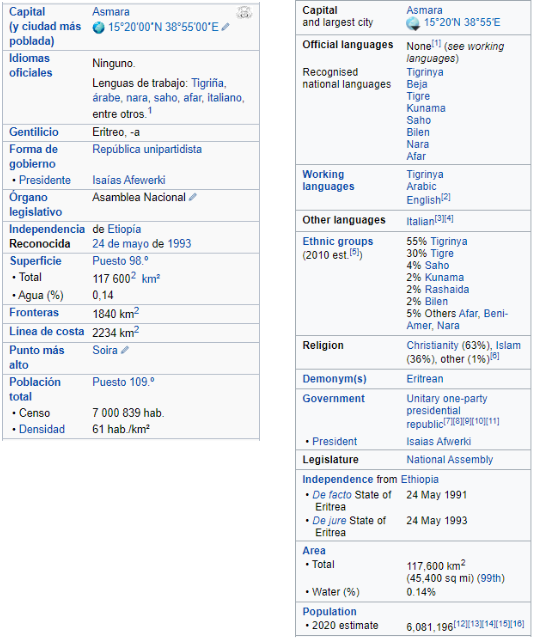
\includegraphics[width=.8\linewidth]{imagenes/EritreaWikipedia.png}
        \caption{Eritrea in both Wikipedia in Spanish and English.}
        \label{fig:eritreaWikipedia}
\end{figure}

Current research is opening many paths for parsing different types of data. In regards to text, a different approach is proposed by the W3C (World Wide Web Consortium). Instead of going from unstructured text to data, the Semantic Web proposes that data can be expressed on the Web in such way that both humans and machines can make use of it. In this proposal, the data is represented in a simple data model structure where common identifiers and standard vocabularies are used to connect the data across different Web domains. With this approach, pages (or parts of pages) could be generated from data and machines would have a better grasp of what the contents are. In the same way, information can be consolidated so that sites present the same information for different language versions.

This architecture proposal, known as the Semantic Web Stack is composed of different hierarchical language layers where higher layers are supported by lower ones (as in an OSI model or similar). As can be appreciated in \Cref{fig:semanticWebStack}, the stack is composed of several layers: a lower layer for identifiers and character set; a syntax layer; a data model layer; a query layer where also taxonomies, ontologies and rules are applied; a unifying logic layer; a proof layer; and a trust layer. All these layers together support user interfaces and applications. A transversal cryptography layer is proposed to support identity verification and encryption of sensitive data. It is important to mention that the stack is under evolution: there are several research proposals for changes to its structure. We will focus on the main layers in this section.

\begin{figure}[H]
    \centering
        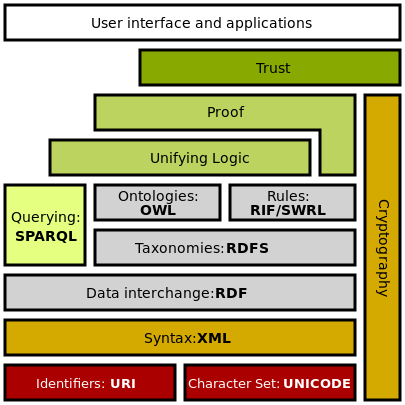
\includegraphics[width=.5\linewidth]{imagenes/Semantic_web_stack.png}
        \caption{Semantic Web Stack \cite{SemanticWebWikipedia}}
        \label{fig:semanticWebStack}
\end{figure}

The lowest layer defines character encoding and identifiers. The Unicode standard is used for character encoding and IRIs (Internationalized Resource Identifier\footnote{An IRI is a generalization of an Unified Resource Identifier (URI) on Unicode.}) for identifiers. This two-part layer supports unambiguous identification of each resource using characters and symbols from different alphabets.

Above this layer sits the syntax layer. This layer defines the grammar and how the identifiers are structured. While XML is the defined standard, N-Triples~\cite{nTriples} and Turtle~\cite{Turtle}  are the most commonly used for syntax and structure. According to their own definitions, "N-Triples is a line-based, plain text format for encoding an RDF graph."~\cite{nTriples} and "Turtle allows RDF statements to be completely written in a compact and natural text form, with abbreviations for common usage patterns and datatypes"~\cite{Turtle}. We can see an example of RDF data in Turtle format in \Cref{fig:turtleExample}. 

\begin{figure}[H]
\begin{minted}[]{sparql}
@prefix ex:    <http://example.org/> .

ex:Earth ex:highestPoint ex:MountEverest .
ex:Asia ex:partOf ex:Earth .
ex:Asia ex:sharesBorderWith ex:Europe .
ex:Europe ex:partOf ex:Earth .
ex:MountEverest ex:continent ex:Asia .
ex:MountEverest ex:namedAfter ex:GeorgeEverest .
ex:GeorgeEverest ex:countryOfCitizenship ex:UnitedKingdom .
ex:GeorgeEverest ex:placeOfDeath ex:London .
ex:UnitedKingdom ex:continent ex:Europe .
ex:UnitedKingdom ex:capital ex:London .
\end{minted}
\caption{Example of RDF data in the Turtle format}
\label{fig:turtleExample}
\end{figure}

In our example, prefixes stay on top of our file and define abbreviations for our data. On the bottom are our subject-predicate-object triples. The same example could be written in N-Triples format.\footnote{To see how these formats compare, the EasyRdf web service: \url{http://www.easyrdf.org/converter} allows users to translate data formats in a simple way.} 

Following the Syntax layer are the data interchange or data model layer and the query layer. We will discuss more about these in \Cref{chap:RDF} and \Cref{chap:SPARQL}. The taxonomies, ontologies and rules layer define how the data fits together: relations and vocabularies are defined in these layers.

On top of these layers we can find the unifying logic, proof and trust logic. While these layers are not completely theoretically defined, they are defined as a proof-of-concept. The unifying logic layer combines ontological reasoning with querying. The proof layer provides a proof of procedures or information to the client, and the trust layer defines access control between services and data.

Regarding the Semantic Web, the state of the art is constantly expanding with new research methods to improve reach, performance or usability in order to bring the Semantic Web closer and closer to users. Some well-known fields where Semantic Web has had notable contributions are drug discovery, patient care management and reporting, publication of scientific knowledge, drug approval procedures, music and movie databases, geospatial data, etc. Interesting works for the author are applications in the industrial sector, for instance where process data from IoT or RFID sensor data is added every second to RDF datastores \cite{Zhang2018,Soylu2018,Kharlamov2016}. In the author's national context, the Chilean Library of Congress has its data available in RDF format~\cite{datosbcn}.

% ##############################################################################################
% ##############################################################################################
% ##############################################################################################


\subsection{Data Model RDF}
\label{chap:RDF}

The Resource Description Framework (RDF) \cite{rdfConcepts, rdfprimer11} is at the core of the Semantic Web. RDF proposes a data interchange model for structuring factual content for interoperability between different data sources (usually the Web, but it can be applied to anything). The goal of the standard is to "facilitate data merging even if the underlying schemas differ, and it specifically supports the evolution of schemas over time without requiring all the data consumers to be changed."~\cite{W3CRDF}. The standard defines RDF terms, triples, graphs and vocabularies. RDF is currently on version 1.1, published in 2014.

An RDF term represents a resource. A resource can either be an IRI, a literal value or a blank node. An IRI is an unambiguous identifier for a resource. Literal values can be text strings or datatypes (integer, boolean, double, datetime, etc.). Literal text strings can be defined in an specific language by adding a language tag: i.e.: "@en" represents a literal text string in English. A blank node (or \textit{bnode}) is used to represent a resource whose identifier or literal is not given. Blank nodes can be seen as denoting anonymous resources.

RDF triples or simply \textit{triples} allow the construction of a statement that relates RDF terms. Three RDF terms can be grouped to create a 3-tuple subject-predicate-object statement: "Mary eats pizza". This format allows for both humans and machines to easily read, query and reason about a data statement. 
In this 3-tuple, the subject identifies which resources the statement is about; the predicate indicates the relationship, traits or aspects between the subject and the object; the object identifies the value of the statement. From this basic 3-tuple structure and using blank nodes, statements can grow in complexity: for example, we can represent the statement "Mary eats (pizza madeOf mozzarella)" using a blank node to represent the pizza.

RDF defines certain grammar rules or semantics \cite{RDFSemantics} for building triple statements:
\begin{itemize}
    \item Subjects must be an IRI or blank node.
    \item Predicates must be an IRI.
    \item Objects can be either an IRI, literal or a blank node.
\end{itemize}

A collection of triples represents a labeled directed multi-graph or simply an RDF \textit{graph}. In RDF graphs, subjects and objects represent nodes and predicates represent labels on directed edges connecting them. In \Cref{fig:bobMarleyExampleGraph} we can appreciate how our RDF data from \Cref{fig:turtleExample} visually looks like.

\begin{figure}[h!]
    \centering
        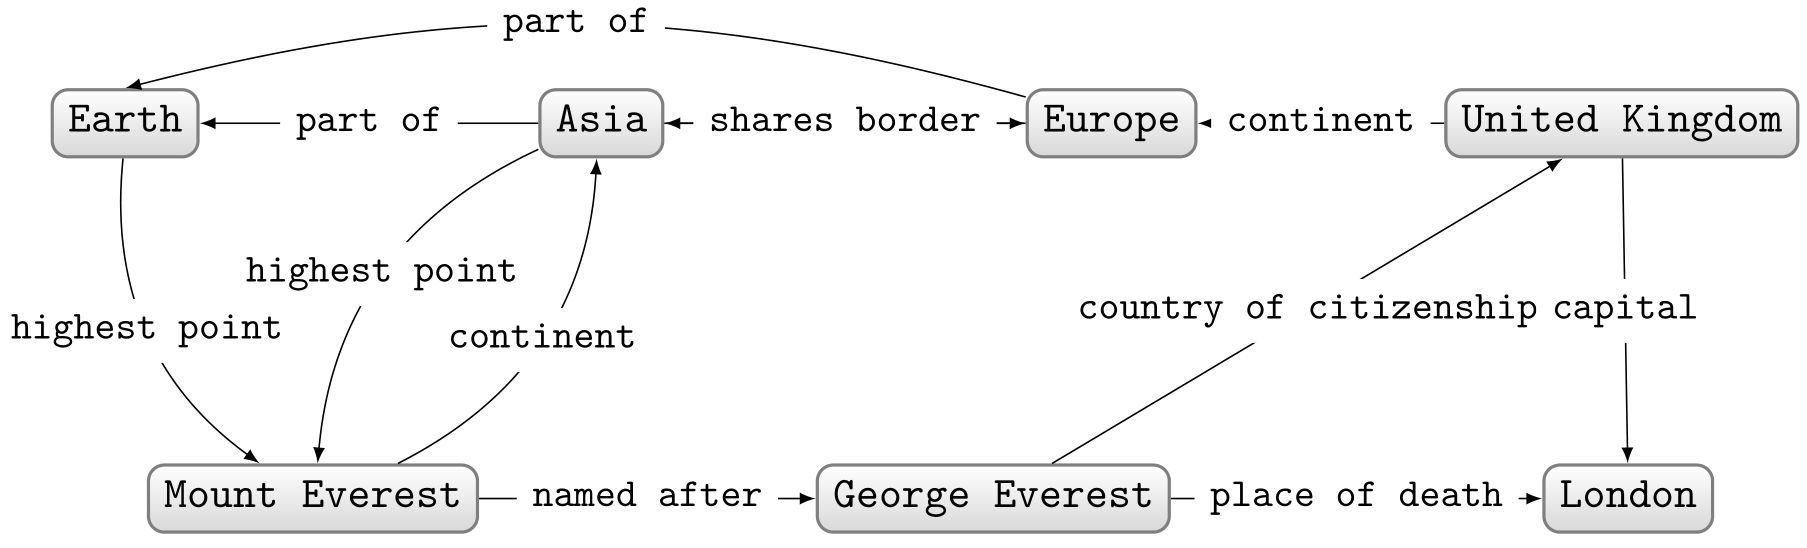
\includegraphics[width=.9\linewidth]{imagenes/exampleGrapha.png}
        \caption{Graph representation of our \Cref{fig:turtleExample} example data~\cite{Moreno2018}}
        \label{fig:bobMarleyExampleGraph}
\end{figure}

RDF vocabularies are built on top of the RDF standard. They add meaning to the relationships within our data. Classes (aka types) and properties (aka relationships) are defined for resources. Classes support class hierarchies, grouping, organization and processing of resources. For example, we may define the classes \textit{City} and \textit{Country} and define them to be subclasses of the more general class \textit{Place}. Properties are extended by the use of vocabularies: ontologies, taxonomies and thesauri are defined to simplify data sharing across diverse applications and enable richer integration and interoperability of data among descriptive communities. Properties may also form a hierarchy, and may have domain and ranges classes to indicate the types of the subjects and objects that they relate. For example, we may define a property \textit{hasCapital} as a subproperty of \textit{hasCity}, both of which have the domain \textit{Country} and range \textit{City}.

Vocabularies are defined in their own standards: RDF Schema (RDFS)~\cite{RDFS}, Web Ontology Language (OWL)~\cite{OWL} and Simple Knowledge Organization System (SKOS)~\cite{SKOS} are powerful technologies to structure and organize data. As per their own reference sites: "RDFS is a general-purpose language for representing simple RDF vocabularies on the Web"~\cite{RDFS}. "OWL is a computational logic-based language such that knowledge expressed in OWL can be exploited by computer programs, e.g., to verify the consistency of that knowledge or to make implicit knowledge explicit"~\cite{OWL}. "SKOS is a common data model for sharing and linking knowledge organization systems via the Web"~\cite{SKOS}. From these vocabularies, we use the following properties in this work: \textit{label}, \textit{alternative label} and \textit{description}. We will not use ontologies and reasoning in this current work, and thus we will not dive deeper into these topics.

% ##############################################################################################
% ##############################################################################################
% ##############################################################################################

\subsection{SPARQL}
\label{chap:SPARQL}

In the previous section we went through the data model to store Semantic Web data. In this section we will focus on how to retrieve this data. SPARQL~\cite{SPARQL} is the W3C standard for querying RDF data. As per the SPARQL reference site: "SPARQL can be used to express queries across diverse data sources, whether the data is stored natively as RDF or viewed as RDF via middle-ware. SPARQL contains capabilities for querying required and optional graph patterns along with their conjunctions and disjunctions. SPARQL also supports extensible value testing and constraining queries by source RDF graph. The results of SPARQL queries can be results sets or RDF graphs."~\cite{SPARQL}

SPARQL uses a syntax similar to SQL (Structured Query Language) for RDF triples. SPARQL query statements are expressed in the RDF Turtle syntax extended with SPARQL keywords. In these statements, clauses are expressed. A clause can contain triple patterns, in which elements of the triple (subject-predicate-object) can be replaced by variables in order to query for specific data.

In our following example, based on our \Cref{fig:turtleExample} example data, we present a simple query on how to get the highest mountain on Earth and in which continent it is located. This query will return the pair \texttt{ex:MountEverest}, \texttt{ex:Asia} because \texttt{?highest} matches in the \texttt{WHERE} clause with \texttt{ex:MountEverest} in the dataset and the same with \texttt{?continent} matching \texttt{ex:Asia}.

\begin{figure}[H]
\begin{minted}[]{sparql}
SELECT ?highest ?continent
WHERE {
    ex:Earth ex:highestPoint ?highest .
    ?highest ex:continent ?continent
}
\end{minted}
\caption{Example of a SPARQL query.}
\label{fig:sparqlQueryExample}
\end{figure}


% ##############################################################################################
% ##############################################################################################
% ##############################################################################################

\subsection{Linked Data}

While the Semantic Web refers to the standards used for storing, relating and querying our human/machine-friendly data, Linked Data is the term used for best practices or principles applied to this data. These principles, according to the reference site~\cite{LinkedData} are as follows:

\begin{itemize}
    \item Use URIs as names for things
    \item Use HTTP URIs so that people can look up those names.
    \item When someone looks up a URI, provide useful information.
    \item Include links to other URIs so that they can discover more things.
\end{itemize}

Using these principles, our goal is to use the Semantic Web standards to represent and access data on the Web, while being able to link (thus the name Linked Data) different resources. The idea is to be able to connect all resources into a global data graph on the Web that users can easily navigate and refer to.

The Linked Data principles have been growing in adoption since their proposal, with multiple community and private RDF datasets available. Many of these Linked Data sites provide clients with user interfaces, APIs and query endpoints for accessing the data using SPARQL or direct navigation. 

A compilation of publicly available linked data sites can be found on \url{https://lod-cloud.net}. Currently the site contains 1,255 datasets with 16,174 links between them (As of May 2020). Datasets in this site are classified in the following categories: Cross-Domain, Geography, Government, Life Sciences, Linguistics, Media, Publications, Social Networking and User-Generated. In this work, we are going to use the Wikidata dataset as our proof of concept~\cite{wikidataQueryService}, but our methods extend likewise to other datasets. We will talk more about this dataset in the following section.

% ##############################################################################################
% ##############################################################################################
% ##############################################################################################

\subsection{Wikidata}

In this work we are going to use RDF data from the \url{https://www.wikidata.org/} site for evaluating our proposal. Wikidata is a free, collaborative, multilingual and open knowledge base that can be read and edited by both humans and machines~\cite{Wikidata2014}. Wikidata acts as central storage for collecting structured data to provide support for Wikipedia, Wikimedia Commons, the other wikis of the Wikimedia movement, and to anyone in the world.

To date, Wikidata describes over 84 million resources with over 5,126 million statements\footnote{\url{https://www.wikidata.org/wiki/Wikidata:Statistics}}. Wikidata resources are uniquely identified by a letter \textit{Q} followed by a number, such as \textit{Douglas Adams (Q42)}. Statements describe detailed characteristics of a resource and consist of a property and a value. Properties in Wikidata have a letter \textit{P} followed by a number, such as with \textit{educated at (P69)}. For Douglas Adams' example, he was educated at the \textit{St. John's College (Q691283)}. The previous example, taken from the Wikidata introduction site, also provides \Cref{fig:wikidataDataModel} to show how this RDF data could be presented to users.

\begin{figure}[h]
    \centering
        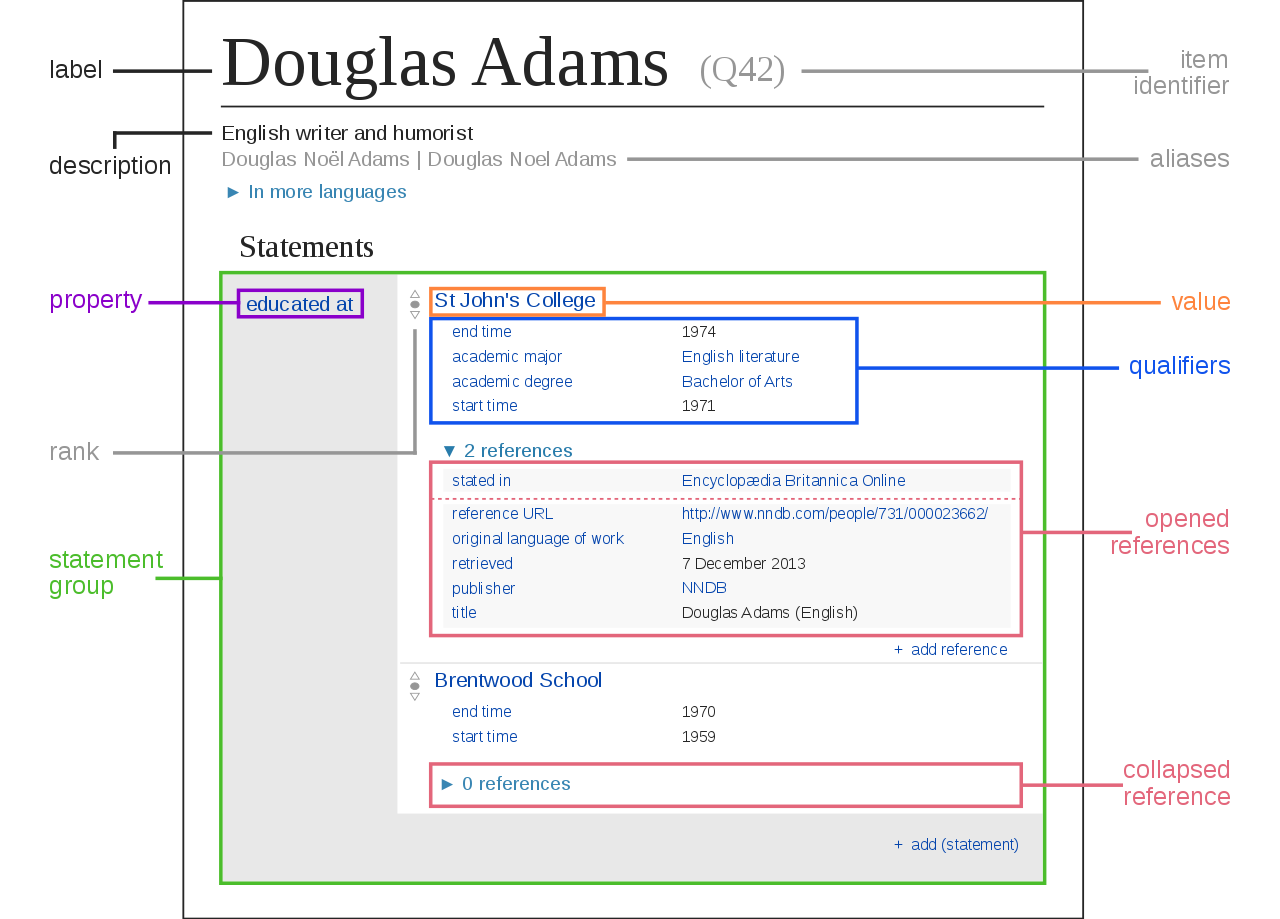
\includegraphics[width=\linewidth]{imagenes/Datamodel_in_Wikidata.png}
        \caption{Wikidata Model. From the Wikidata introduction site~\cite{WikidataIntroduction}}
        \label{fig:wikidataDataModel}
\end{figure}

It is possible to download a copy of the whole Wikidata knowledge base in RDF/N-Triples format. This 41 GBytes compressed RDF dump contains the previously mentioned information as RDF triples. The RDF triples that model the previous example are presented in \Cref{fig:rdfDataExample}. This data is publicly available at the \url{https://dumps.wikimedia.org/wikidatawiki/entities/} site. While it is possible to instantiate different SPARQL engines to query this database~\cite{Hernandez2016}, we will be working with the plain N-Triples data dump. For querying purposes, we will use the Wikidata API available at \url{https://www.wikidata.org/w/api.php}.

\begin{figure}[H]
\begin{minted}[]{sparql}
# Single line comments begin with the '#' character
# Label
wd:Q42 rdfs:label "Douglas Adams"@en . 
# Alternative labels
wd:Q42 skos:altLabel "Douglas N. Adams"@en .
wd:Q42 skos:altLabel "Douglas Noel Adams"@en .
# Description
wd:Q42 schema:description "English writer and humorist"@en .
# Properties, such as place of birth (P19), country of citizenship (P27), 
# instance of (P31), educated at (P69) and residence (P551).
# The next line reads: Douglas Adams' place of birth is Cambridge (Q350).
wd:Q42 wdt:P19 wd:Q350 .
wd:Q42 wdt:P27 wd:Q145 .
wd:Q42 wdt:P31 wd:Q5 .
wd:Q42 wdt:P69 wd:Q691283 .
wd:Q42 wdt:P551 wd:Q84 .
\end{minted}
\caption{Example RDF data for Douglas Adams in Wikidata (Q42).}
\label{fig:rdfDataExample}
\end{figure}

% ##############################################################################################
% ##############################################################################################
% ##############################################################################################

\section{Information Retrieval}

In the previous section we introduced some key Semantic Web concepts. While these concepts will be relevant in terms of the type of information that we process, we require techniques from another field of Computer Science to  be able to process and manage this information. The field called Information Retrieval is concerned with finding information from large collections. In order to find this information, this field uses indexes and relevance measures to store and classify the information. For our work, we will be using Inverted Indexes to store and search information, while using Term-Frequency-Inverse-Document-Frequency (TF-IDF) and PageRank for ranking the results.

\subsection{Inverted Index}
\label{chap:lucene}

In our research we take information about Semantic Web resources described using RDF and store it in an specialized index. In this index, we will store information about RDF resources, such as the identifier (subject id), the label, description, alternative labels, outgoing properties (predicates available) and so on. This information is extracted from the triples associated with a resource. We will go into more detail on this in \Cref{chap:index}.

Since much of the information that we are going to index is text based, a suitable index is an inverted index. In a forward index, like relational databases, each resource is stored by its id and all available fields are accessed through that id. In an inverted index, fields are stored and the resource ids are accessed by searching over the fields. Inverted indexes are commonly used for text document indexing, where a collection of words are indexed. Every time a user searches for something, they will query these words and the documents containing them will be returned as results.

In this work we will build a document for every resource described by the RDF graph, where our label, alternative labels and descriptions will work as our different text fields. With this index, we will be able to search for words, such as "\textit{capital of Seychelles}" and as an answer we would get all documents that contain these words. Among the results we will get \textit{Victoria} and also \textit{Seychelles} (while also getting other capital-related documents). In order to get this to work properly, our index will deal with different kinds of fields:

\begin{itemize}
    \item Text fields contain text and ignore stop words and group similar words.
    \item Numeric fields allow us to store integers or doubles, while providing support for sorting and range queries.
    \item String fields look for exact matches, such as the name of our resource subject name.
    \item Stored fields allow us to save information that is not required for querying, such as our predicates.
\end{itemize}

There are two more points worth mentioning for inverted indexes. Since we are processing some of the input data while building our index, inverted indexes take longer to create than forward indexes. The other point is relevance: Inverted indexes can sort the queried results by certain criteria: 

\begin{itemize}
    \item Matching a word in the label of a document might be more relevant than matching a word in the description of it.
    \item Rare words that might appear less frequently in the collection of documents boost the relevance of our results.
    \item Matching several words in our query pattern might also bump the relevance of our results up.
    \item Words occurring more frequently in a document indicate higher relevance.
\end{itemize}

A ranking measure based on these criteria is known as TF-IDF and is one of the ranking measures that we will implement for our text-based lookups. In the following section, we will cover how TF-IDF is not the only measure that we will implement and we will also cover why another measure is helpful.

% ##############################################################################################
% ##############################################################################################
% ##############################################################################################

\subsection{Ranking}
\label{chap:pagerank}

In the previous section we mentioned which indexing method we will use and how it inherently implements a ranking measurement for sorting query results. We mentioned that, while this TF-IDF is in place, another ranking measure may help our users to get better results.

Let us take for example "Jordan". On the one hand we have the country, while on the other we have the basketball player. If you go to Google and search for Jordan, what would you expect to be shown first? This is a hard question to answer. In order to estimate the resources relevant to a keyword search that a user is most likely to be interested in, an importance metric algorithm is implemented next to our relevance ranking metric: based on how many references links-to and how many other resources are linked-from a resource, an importance ranking value can be set to better optimize results.

A similar approach for link-based ranking, proposed in 1998 by Google's founders Larry Page and Sergey Brin, is known as PageRank~\cite{Page1998}. It was first conceived to add importance ranking to web sites. In their proposal, web sites are modelled as a directed graph: Each web site is a node, web sites may have incoming links (links that direct to that site) and outgoing links (links that direct to other sites). After modelling the web like this, a recursive algorithm takes place: A page with lots of inlinks from important pages with few outlinks is more important. There are some scenarios to consider: when a document has no links and when two documents link only to each another. In order to avoid high relevance from these cases, there is a probability to not follow any link and jump to a random document.

The PageRank process sets an initial value to all documents: this value is the same for all, such that the sum of all document’s rank is 1. The next step will be to share the document's rank to all documents it links to: a higher ranked document gives a higher rank to its links, while documents with lots of links give a low rank because its rank is divided across all its links. With the probability to jump randomly (usually set as 0.15), this process is recursive and guarantees to converge, so after a number of iterations each document’s rank is fixed.

For our research, we are not dealing with web sites but with RDF resources that link to other RDF resources, thus this application also fits our needs. PageRank will work by considering the incoming and outgoing edges between RDF resources (see \Cref{fig:bobMarleyExampleGraph}) as the incoming and outgoing links in web sites. Using both our PageRank importance and the TF-IDF relevance, query results are sorted and returned to our users. This approach can be used to rank the nodes of an RDF graph, namely the terms appearing as the subject and/or object of one or more triples. However, PageRank is not directly applicable to rank property terms. In order to rank properties, we rather use the frequency of the property in terms of how many triples in the RDF graph use that property. We assume that users will often be interested in properties that are most frequently defined in the data.

% ##############################################################################################
% ##############################################################################################
% ##############################################################################################

\section{User Interfaces}

In \Cref{chap:SPARQL} we covered SPARQL, the W3C standard for creating RDF queries. While this approach serves the purpose of creating queries, it requires an understanding of both the SPARQL language syntax and the underlying RDF data structure: which properties exist and how they interrelate resources. As we mentioned before, other authors have identified that these are two main issues limiting Semantic Web adoption by non-technical users: SPARQL language syntax and the lack of helpful user interfaces~\cite{Ferre2016, Lehmann2014, Unger2014}.

The third field of Computer Science that will take part in our research will be User Interfaces. How will our users engage with our system? How will we support their journey of using Linked Data? There are two pieces that fit our work: We will use visualization and query interfaces to help users explore, navigate and create SPARQL queries in an interactive way (without dealing with SPARQL); and we will use autocomplete to support the selection of results from a collection of candidate suggestions. 

Autocomplete or picklists allow users to narrow a collection of results by typing characters that get the users closer to their desired result. There are several techniques that can be implemented under an autocomplete user control. Fuzzy search or approximate string matching is a technique to find strings that match a pattern approximately, rather than exactly. Debounce timers allow autocomplete user controls to wait some time before submitting a query: this makes the system more fluent, skipping immediate changes (like adding/removing single characters) and waiting for users to elaborate on their query terms before firing another search event.

In other application fields, autocomplete can be easily be implemented since the scope is relatively fixed or small. In relational databases the structure or schema of the database is fixed independent of the size of the database. While the schema can change, its modifications are not as dynamic as the data itself. In IDEs on the other hand, the source code structure is dynamic, but the size of this structure is not a problem for a modern IDE and changes are handled on the go. This autocomplete indexing process can be experienced when importing a large codebase into a modern IDE. The system will require several minutes before any suggestions can be provided. In contrast with relational databases, RDF graphs do not have something analogous to a relational schema, likewise the scale of RDF graphs is often greater than the scale of a codebase.

Visualization and query interfaces aim to help users navigate, explore and build queries without necessarily writing code by means of displaying resources and connecting them in an easy-to-use visual user interface. These systems also support users in navigation tasks, by displaying information of a subject and its relation with others. Most such systems are designed for a specific language. While there are multiple recommendations and studies related to these types of user interfaces~\cite{Dadzie2011, Bikakis2016}, there are no defined rules or standards that guide the development of these systems. In the following section we will cover some of the existing research work available for these topics in the context of RDF data.

With regards to visualization and exploration of RDF data, we have studied two surveys that cover this topic. Dadzie et al.'s work: "Approaches to visualising Linked Data: A survey"~\cite{Dadzie2011}, studies several existing systems, classifies and evaluates them according to their scalability, as well as their features for filtering, data overview, text/graph view, faceted search, among others. Their statement is that for users to better understand the underlying structure of RDF triplestores, a key solution "is to visualise Linked Data in a coherent and legible manner, allowing non-domain and non-technical audiences to obtain a good understanding of its structure, and therefore implicitly compose queries, identify links between resources and intuitively discover new pieces of information."

A follow-up survey conducted in 2016 by Bikakis et al.: "Exploration and Visualization in the Web of Big Linked Data: A Survey of the State of the Art"~\cite{Bikakis2016} makes a sweep through the state of the art systems for exploration and visualization. 
Their work states how "exploring and visualization of very large dataset has become a major research challenge, of which scalability is a vital requirement". They also describe some major prerequisites and challenges that should be addressed by modern exploration and visualization tools.
In their research, they identify that most traditional exploration and visualization tools operate in an offline way, limited to small datasets, and not being able to explore large-scale datasets, such as the one that we will be using in this work.

Regarding autocomplete, some authors have approached the idea of adding autocomplete support to SPARQL queries. 
In their research work "Designing scientific SPARQL queries using autocompletion by snippets" Rafes et al.~\cite{Rafes2018} have conducted a two year study on SPARQL queries expressed by a community of scientific users. 
In this work they have studied different text query editors\footnote{Flint Editor, iSPARQL, LODatio+, BioCarian, Gosparqled, Wikidata Query and YASGUI. All cited by Rafes et al.~\cite{Rafes2018}} with autocomplete features and classified them into four main techniques: 
\textit{Autocompletion using relative IRIs via keywords}; 
\textit{Autocompletion by prefix declaration}; 
\textit{Autocompletion by template}; and 
\textit{Autocompletion by suggestion of snippets}. 
They have also identified that users usually fail to express SPARQL queries due "to imperfect knowledge on the ontologies involved in the queries or the need to follow a syntax rather complex to master"~\cite{Rafes2018}. 
Their work is based on "suggesting fragments of queries made by other previous users to complete the partial query already written by the user"~\cite{Rafes2018}.
It works by "extracting representations of subpatterns from previous queries (in the form of 'linegraphs') and construct a hierarchical clustering of such subpatterns to generate snippets that are most compatible with the portion of the query considered by the user"~\cite{Rafes2018}. Our methods are similar in that we provide suggestions to users, but based on the data that exists in the triplestore itself.

Another approach to autocompletion has been proposed by El-Roby et al.~\cite{El-Roby2016}. 
In their work "Sapphire: Querying RDF Data Made Simple", they propose "a tool that helps users write syntactically and semantically correct SPARQL queries without prior knowledge of the queried datasets."~\cite{El-Roby2016}
In their study, they have identified that Natural Language approaches for querying are good for simple queries, but not for complex queries. 
For complex queries, they remark that "the user needs to know the structure of the dataset, the vocabulary used to represent different concepts, and the literals used in the dataset including their data types and format."~\cite{El-Roby2016}
Their system "provides data-driven suggestions to complete the predicates and literals in the query"~\cite{El-Roby2016}. 
As in our work, their architecture is based on a server that sits between the user and the SPARQL endpoint.
The indexing mechanics between Sapphire and our work differ mainly on two points: 
They build their index with a sample of the data, built by running multiple queries (17 hours of queries for DBpedia), on the remote endpoint for hierarchical relations and predicates; 
the second difference is that their proposals are based on properties that point to literals and not entity-to-entity relations.

There are a couple of visual query/exploration systems that we found interesting in the context of this work: "VIQUEN: A visual query engine for RDF" by Dell~\cite{Dell2010}, "Node-centric RDF Graph visualization" by Sayers~\cite{Sayers2004}, "ViziQuer: a Web-based tool for visual diagrammatic queries over RDF data" by Cerans et al.~\cite{Cerans2018}, "FedViz: A Visual Interface for SPARQL Queries Formulation and Execution" by ~\cite{Zainab2015}, among others. From studying these works, we have noted that some rely either on domain specific, offline local triplestores, SPARQL-syntax-based queries or direct-to-endpoint queries for data retrieval. These works set important precedents for exploration and navigation of triplestores.

The visual query system "Smeagol: A 'Specific-to-General' Semantic Web Query Interface Paradigm for Novices" by Clemmer et al.~\cite{Clemmer2011} helps users to build queries that "guides the user from a specific example to a general result set". This novel approach is very helpful since it allows users to navigate and explore the data until they build a concrete subgraph of interest which then can be generalized to find other subgraphs similar to the one identified. Their work provides some interesting features such as autocompletion, dynamic results (query results are generated and used during query construction, which in turn helps building a better query), and non-emptiness guarantees. We find two drawbacks on their work: their system is only able to build tree-shaped queries and does not support general graph patterns; and their exploration tasks are done directly over the remote SPARQL endpoint, which faces the problems described before.

Vargas et al. in their "RDFExplorer: A Visual SPARQL Query Builder" research take Smeagol as a base system to develop further. Their work, as we mentioned before, supports users in navigation and query building tasks while displaying dynamic results during query building. We have found their interface to be very easy to use and supports keyword lookups for entities and properties with autocomplete features. An improvement upon Clemmer's work is that this research supports multiple graph patterns with cycles. Still, the system gets the suggestions by querying the endpoint directly, which can end in timeouts for many user queries. An additional advantage of this research, is that the source code is publicly available at \url{https://github.com/hvarg/RDFExplorer} while also having a live version available at \url{https://www.rdfexplorer.org/}.
\chapter{System Overview}
\label{chap:overview}

In this chapter we present an overview of our system. 
We will start by providing an overall description of the system: 
the main components and how these relate to each other. 
This will be followed by the possible user interactions: 
the different types of queries that can be requested to our backend as well as how these requests are handled.

In this section we intend for readers to get a general overview of the work; we will go into finer detail for the individual components in \Cref{chap:Backend} and \Cref{chap:Frontend}.

\section{System Architecture}

Our system architecture is as depicted in \Cref{fig:architecture}.

\begin{figure}[H]
    \centering
        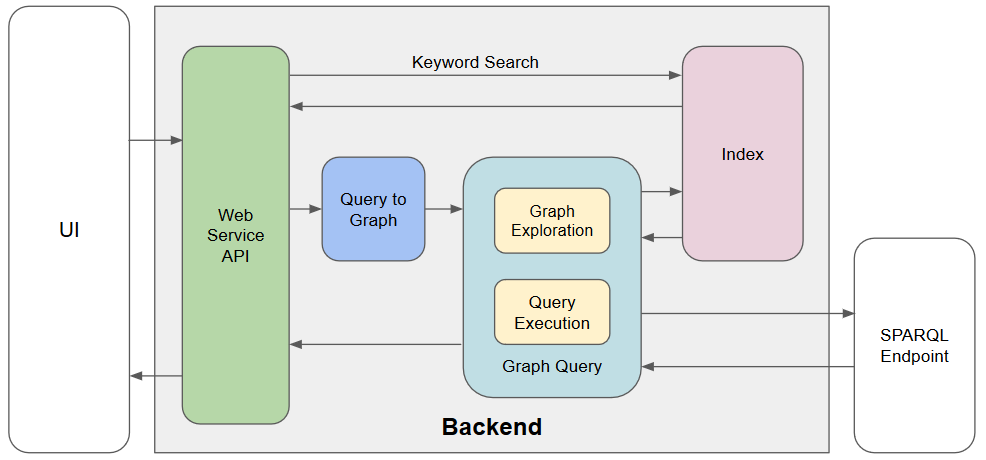
\includegraphics[width=\linewidth]{imagenes/architecture.png}
        \caption{System Architecture.}
        \label{fig:architecture}
\end{figure}

Our system allow users that are building SPARQL queries to get entity and property suggestions from a triplestore. 
This works in two ways: 
A first contribution is to allow users to query entities or properties via keyword search. 
The second and most important contribution of our work is to provide suggestions for SPARQL terms, based on the query that is being built. 
All given suggestions are sorted by relevance and importance.

Our system is built entirely as a web service backend. 
This backend sits between the user interface and a remote SPARQL query endpoint. 
The entry point of our system is an API that will take requests from different services, such as SPARQL query editors or SPARQL visual explorers. 

Depending on the query type, the system can do a keyword search directly on the index, or it can parse the query for SPARQL triple patterns. 
In the latter case, the SPARQL query will be converted to a graph. 
This graph will be processed and then sent for execution. 
The execution of the query is sent in parallel to both the remote SPARQL endpoint and the local index. 
The results are then post-processed and sent back to the user for display and selection. 
We will expand some more on these steps in the following sections.

These last interactions, related to the UI, are not in the scope of our work; nevertheless, we have integrated our system to a visual query system for demonstration. 
This UI integration, both for the request and the display of results, is explained in detail in \Cref{chap:Frontend}.

It is important to mention that before our system can provide results, it has to be initialized with an RDF dataset dump. 
This initialization process can be divided into two sub-processes: 
Pre-processing and Indexing. 
The details of this initialization are described in \Cref{chap:init}. 

All the source code for the back-end is written in \textit{C\#} as a .Net Standard Library. 
The following dependencies are used:

\begin{itemize}
    \item \textit{Lucene.Net}\footnote{\url{https://lucenenet.apache.org}} is used for the index. 
    \item \textit{DotNetRDF}\footnote{\url{https://www.dotnetrdf.org}} is used for handling, reading and writing RDF.
    \item \textit{SharpZipLib}\footnote{\url{http://icsharpcode.github.io/SharpZipLib}} is used for handling compression.
    \item \textit{Mime}\footnote{\url{https://github.com/hey-red/Mime}} is used for identifying file types checks.
    \item \textit{xUnit}\footnote{\url{https://xunit.net}} is used for Unit Testing.
    \item \textit{NLog}\footnote{\url{https://nlog-project.org}} is used for logging.
    \item \textit{ASPNetCore}\footnote{\url{https://docs.microsoft.com/en-us/aspnet/core}} is used for the Application Interface (API).
    \item \textit{Newtonsoft.Json}\footnote{\url{https://www.newtonsoft.com/json}} is used for handling JSON.
\end{itemize}

The integration code for the front-end is written in \textit{JavaScript}. The code is available at the following locations:
\begin{itemize}
    \item \url{https://github.com/gabrieldelaparra/SPARQLforHumans}. This project.
    \item \url{https://github.com/gabrieldelaparra/RDFExplorer}. Forked and modified version of RDFExplorer.
    \item \url{https://github.com/hvarg/RDFExplorer}. RDFExplorer~\cite{Vargas2019}.
\end{itemize}

\section{User Interactions}

As mentioned before our system has two different ways for users to request information: 
Keyword search 
and SPARQL query term suggestions.

\subsection{Keyword search}

The keyword search feature enrich the user experience of RDF datasets by providing lookup access via \textit{labels}, \textit{descriptions} or \textit{alternative labels} for the queried data. 
Keyword search functionality is one of the most natural ways of looking for information. 
While this feature is the de-facto way for users to search for something (e.g. DuckDuckGo) it is not included as part of the SPARQL standard. 
Keyword search allows users with no or limited knowledge of prefixes or ids to get to their desired results. 
The keyword search mechanics are quite straightforward; a keyword request is sent to the backend and a list of possible entities or properties, sorted by relevance, are returned. 

\begin{example}
A user wants to search for the type \textit{Human} in the Wikidata dataset. 
They could have no idea that \textit{wd:Q5} is the identifier for this entity. 
They could search for \textit{"person"} or \textit{"people"} instead. 
Since \textit{person} and \textit{people} are alternative labels for \textit{Human}, the latter is displayed in the results. 
As per the results, \textit{Human} is displayed before \textit{Grammatical Person}, since human is deemed to be more likely to be of relevance to the user, and thus is given a higher order than what the alphabetic order would sort.
\end{example}

\begin{example}
A user would like to search for the \textit{head of government (wdt:P6)}  property, once again, in the Wikidata dataset. 
As keywords, the user could enter \textit{"president"}, \textit{"mayor"} or \textit{"prime minister"}, since this would be a more natural way of looking for that property, depending on the user and query context. Once again, suggestions including \textit{head of government} are returned and ordered by a measure of how likely they are to be relevant to the user.
\end{example}

\begin{example}
A user is trying to search for \textit{Reykjavík}. 
Since typing the name correctly would be a challenge for certain users, this author included, the \textit{"capital (of) Iceland"} could be used to search. 
Since the system has been indexed for \textit{descriptions}, the desired result would appear as the first result. 
\end{example}

\subsection{SPARQL query term suggestions}

The term suggestions help users to create SPARQL queries. 
A SPARQL query is composed of multiple triple patterns.
As seen in \Cref{chap:SPARQL}, a triple pattern can be something like \textit{"Mary eats pizza"}. 
Lucky Mary. 
Each triple in the SPARQL grammar is composed of three terms: 
a \textit{subject} (\textit{"Mary"}), 
a \textit{predicate} (\textit{"eats"}) 
and an \textit{object} (\textit{"pizza"}). 

We will now briefly describe this process' overview; the details will be revised in more detail in \Cref{chap:Backend}. 
We will accompany this description with some examples about the delicious pizza Mary was eating.

Query construction starts by supposing that a triple pattern is always available, even when there are only variables, such as in \textit{?var1 ?prop1 ?var2}. However, triple patterns will often contain specific terms in combination with variables, as seen in the previous example.

As a first step, an application uses our service for getting suggestions. 
The user of this application still has not added anything to its query. 
For a blank string, a triple pattern with only variables is added. 
The following triple pattern represents the current query:

\begin{minted}[escapeinside=||,frame=none,linenos=false]{text}
    ?var1 ?prop1 ?var2 .
\end{minted}

During query construction, a user will start adding terms to their triple patterns. 
At this stage, if everything is a variable, the keyword search will return results. 
In this context, a user might start by typing \textit{"Ma"} and several suggestions will be displayed. 
For this example, the results will include \textit{"Mary"}, \textit{"Marocco"} or \textit{"Mango"}. 
The user selects \textit{"Mary"} between the suggestions and \textit{Mary} is added to the query as the \textit{subject} term. 
The system recognizes that \textit{Mary} is of type \textit{Human}. The triple should now look like this:

\begin{minted}[escapeinside=||,frame=none,linenos=false]{text}
    |\bf{Mary}| ?prop1 ?var2 .
\end{minted}

Next the user moves to the \textit{predicate} \texttt{?prop}. 
The user will get suggestions like \textit{"eats"}, \textit{"parent of"} or \textit{"studies at"}, which are defined on subjects of type \textit{Human} in the data, but not \textit{"capital of"}, which is not defined on any subject of type human in the data. 
The user selects \textit{eats}. The predicate is replaced with that property. 
The query at this stage looks like:

\begin{minted}[escapeinside=||,frame=none,linenos=false]{text}
    |\bf{Mary}| |\bf{eats}| ?var2 .
\end{minted}

Next the user moves to the \textit{object}, which is a variable. 
Several suggestions like \textit{"cake"}, \textit{"tofu"}, etc. are displayed. 
The user can type in \textit{"pi"} and will be suggested \textit{"pie"}, \textit{"pizza"}, \textit{"pineapple"}, etc., but not \textit{"pillow"} or \textit{"pictures"}, etc., as these are not eaten by anything in the data, nor \textit{"pine cones"}, \textit{"pigeons"}, etc., which though eaten in the data are not eaten by instances of \textit{Human}.

This process might continue until the user has finished building the query. 
At any stage the user can leave a term as a variable and query for all the values that the variable takes.
The user can also join statements, creating more complex queries.

Behind the curtains, during this query construction process the input data is read from the SPARQL query, parsed and stored into a data structure for further processing. 
Our system will convert that query into a graph. 
More about the conversion between SPARQL query and such graphs will be covered in \Cref{chap:parser}.

This graph will be then explored to check for relations between the nodes and the edges. 
Each of the nodes and edges will be classified as either variables, given types or inferred types. 
If other statements are given at this stage, a decision process involving given-types and intersections between inferred types for different incoming/outgoing properties would occur. 
This helps the system to correctly assign types based on the explicitly given ones and the inferred ones. 
All of this will be covered in more detail in \Cref{chap:graph_exploration}.

Once all nodes and edges have been classified, the information will be requested in parallel threads from both sources: 
Local Index and Remote SPARQL Endpoint. 
The request to the remote endpoint is sent with a configurable timeout, usually of a few seconds. 
If the remote endpoint returns values within this time, this results will be returned; otherwise, our internal local index results will be returned. The local results will only be returned if the remote endpoint request fails/times-out. 
This double request mechanism allow us to suggest possible results that would otherwise keep the user indefinitely waiting or in the worst case, never return. 
More on this in \Cref{chap:execution}.

Once the results are consolidated, they will be returned to the UI which made the request. 
For testing purposes, we have integrated our system within an existing visual SPARQL building frontend. 
This integration is described in \Cref{chap:Frontend}.

Before ending this chapter, we would like to emphasize something that was mentioned before. 
Our system can provide approximate results for some triple patterns in complex queries. 
We will try to explain these approximations by example. 
Consider that in our input dataset, there is no such triple for Mary (Mary eats Pizza), but that triple does exist for Bob (Bob eats Pizza). 
While constructing a complex query, where the remote endpoint times out, the local index results for an instance of type \textit{Human} and for the \textit{eats} predicate, will return Pizza as one of the alternatives.
This is due to the nature of our index.
Our index is not based on complete triples, but types, domains and ranges.
This way of indexing supports the query term suggestion tasks, but approximates results for such cases.
\chapter{Autocompletion Techniques}
\label{chap:Backend}

In this chapter we describe the details of our system. Per \autoref{fig:architecture}, our implementation works as a backend that sits between the user interface and a remote SPARQL query endpoint. It takes SPARQL queries as input and returns suggestions for the variables in those queries. Since we are focusing on dealing with large datasets (480GB for the uncompressed Wikidata dump), direct in-memory storage/query is not possible; rather a specialized on-disk index is required.  Before we describe the details of our backend, we introduce an extended example in order to provide an overview of the system.

\section{Overview}

Let us consider that a user is looking for "siblings that have directed a film together". 
Since the user might not very familiar with the available properties in a dataset such as Wikidata, it would be hard for them to directly specify the properties they require. Since they might not be familiar with SPARQL syntax it might be even harder for them to specify the required query directly on the SPARQL endpoint. Rather they choose to use a graphical query builder, like RDFExplorer~\cite{Vargas2019}. Let us consider that they have built a graph query such as the one in \autoref{fig:siblingsQueryGraph}:

\begin{figure}[H]
    \centering
        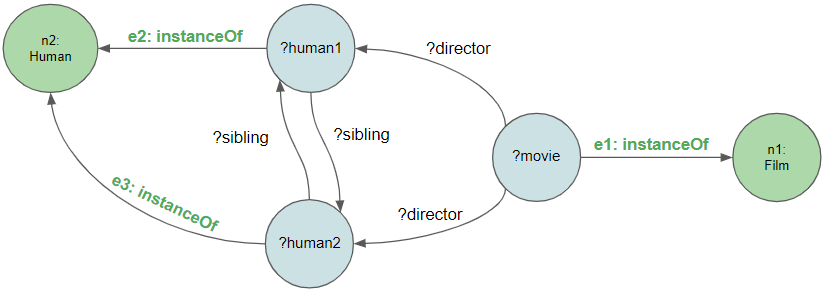
\includegraphics[width=\linewidth]{imagenes/SiblingsGraph.png}
        \caption{Example graph: siblings that have directed a film together}
        \label{fig:siblingsQueryGraph}
\end{figure}

For the example given in \autoref{fig:siblingsQueryGraph}, let us consider that some RDF triples, such as the ones presented in \autoref{fig:siblingsRDFdata}, exist. 

\begin{figure}[H]
\begin{minted}[]{sparql}
[...]
ex:LanaWachowski ex:instanceOf ex:Human . 
ex:LanaWachowski ex:siblingOf ex:LillyWachowski . 
[...]
ex:LillyWachoski ex:instanceOf ex:Human . 
ex:LillyWachoski ex:siblingOf ex:LanaWachowski . 
[...]
ex:Matrix ex:instanceOf ex:Movie .
ex:Matrix ex:directedBy ex:LanaWachowski . 
ex:Matrix ex:directedBy ex:LillyWachoski . 
[...]
\end{minted}
\caption{Example of the underlying RDF data for the query in \autoref{fig:siblingsQueryGraph}.}
\label{fig:siblingsRDFdata}
\end{figure}

Depending on the Linked Data source that is used (e.g.: DBPedia, Wikidata) triples may have different identifiers and namespaces. In \autoref{fig:siblingsWikidataRDF} we present the Wikidata representation for these triples.

\begin{figure}[H]
\begin{minted}[]{sparql}
[...]
wd:Q9545711 rdfs:label "Lana Wachowski"@en .
wd:Q9545711 wdt:P31 wd:Q5 . # Instance of Human
wd:Q9545711 wdt:P3373 wd:Q9544977 . #Sibling Lilly Wachowski
[...]
wd:Q9544977 rdfs:label "Lilly Wachowski"@en .
wd:Q9544977 wdt:P31 wd:Q5 .  # Instance of Human
wd:Q9544977 wdt:P3373 wd:Q9545711 . #Sibling Lana Wachowski
[...]
wd:Q83495 rdfs:label "The Matrix"@en .
wd:Q83495 wdt:P31 wd:Q11424 .  # Instance of Film
wd:Q83495 wdt:P57 wd:Q9545711 . # Director Lana Wachowski
wd:Q83495 wdt:P57 wd:Q9544977 . # Director Lilly Wachowski
[...]
\end{minted}
\caption{Example of the Wikidata RDF data representation of \autoref{fig:siblingsRDFdata}: proper identifiers and namespaces are used.}
\label{fig:siblingsWikidataRDF}
\end{figure}

Without knowing the resource identifiers, or knowing a few of them, and using the Wikidata Query Service~\cite{wikidataQueryService} a user might create a query that could be something like in \autoref{fig:siblingsSPARQL}. 
For the example query, we have added some of the basic identifiers, such as \texttt{wdt:P31} (\textit{instanceOf}), \texttt{wd:Q5} (\textit{Human}) and \texttt{wd:Q11424} (\textit{Film}), but these might also be variables\footnote{We differentiate constant from variables: a constant in our example would be Human (Q5) or instance of (P31). All the other elements, starting with '?' are variables. Our system will propose results only for variables.}. 
In such a case, users could search values to replace variables via keyword lookup (or leave them as variables and use our system to select a value). 
We have added these values to further explain our backend. We have also added some properties, such as \texttt{?sibling} and \texttt{?director} as variables; we will explain how a user can get suggestions for these variables.
We remark that in practice these variables will likely have generic labels such as \texttt{?var1}, \texttt{?var2}, etc., where we add variables with more intuitive labels for illustration purposes. 
We would also like to note that some relations, like director, can be a tricky. One could think that the relation is in the other way: e.g.: \texttt{?human directed ?movie}. We will discuss more about this in our future work section \autoref{chap:futureWork}.

\begin{figure}[H]
\begin{minted}[]{sparql}
SELECT * WHERE {
    # ?human1 and ?human2 are instances of (P31) Human (Q5)
    ?human1 wdt:P31 wd:Q5 .
    ?human2 wdt:P31 wd:Q5 .
    
    # ?movie is an instance of (P31) Film (Q11424).
    ?movie wdt:P31 wd:Q11424 .
    
    # ?human1 and ?human2 are ?siblings.
    ?human1 ?sibling ?human2 .
    ?human2 ?sibling ?human1 .
    
    # ?movie has as ?director both ?human1 and ?human2.
    ?movie ?director ?human1 .
    ?movie ?director ?human2 .
}
\end{minted}
\caption{Without some knowledge the underlying RDF data, a user could create a query where the properties are variables. A query like this will time out in a SPARQL endpoint such as \url{https://query.wikidata.org/}}
\label{fig:siblingsSPARQL}
\end{figure}

The purpose of our system will be to guide users in going from the previously constructed query in \autoref{fig:siblingsSPARQL} to a more complete query such as in \autoref{fig:siblingsSPARQLFull}.

\begin{figure}[H]
\begin{minted}[]{sparql}
SELECT * WHERE {
    # ?human1 and ?human2 are a Human (Q5), ?movie is a Film (Q11424).
    ?human1 wdt:P31 wd:Q5 .
    ?human2 wdt:P31 wd:Q5 .
    
    ?movie wdt:P31 wd:Q11424 .
    
    # ?human1 and ?human2 are siblings (P3373).
    ?human1 wdt:P3373 ?human2 .
    ?human2 wdt:P3373 ?human1 .
    
    # ?movie was directed by (P57) both ?human1 and ?human2.
    ?movie wdt:P57 ?human1 .
    ?movie wdt:P57 ?human2 .
}
\end{minted}
\caption{Our system can provide users with suggestions for entities and properties, so that they can easily identify resources.}
\label{fig:siblingsSPARQLFull}
\end{figure}

Our system can also provide suggestions for \texttt{?human1}, \texttt{?human2} and \texttt{?movie} (such as \textit{Lana Wachowski}, \textit{Lilly Wachowski} and \textit{The Matrix}); which is not what we need in the current scenario, but could be in other scenarios. Once a query is shaped as presented in \autoref{fig:siblingsSPARQLFull}, it can be evaluated to get values for these variables. The query expressed in \autoref{fig:siblingsSPARQLFull} can be run directly on a SPARQL endpoint such as \url{https://query.wikidata.org/} and to date, 125 siblings will be displayed as results. Likewise, we could in theory run the query in \autoref{fig:siblingsSPARQL} over the SPARQL endpoint to generate results, and thus return suggestions for replacing individual variables towards constructing the query of \autoref{fig:siblingsSPARQLFull}. However, the query of \autoref{fig:siblingsSPARQL} times out on the public Wikidata endpoint: with so many variables, it generates too many intermediate results for the endpoint to process in the time limit of 50 seconds. For this reason we propose methods to generate approximate suggestions to replace individual variables of such queries.

For our system to work (in order to get from \autoref{fig:siblingsSPARQL} to \autoref{fig:siblingsSPARQLFull}), first our specialized index must be built and then queries will be processed. Our index differs from a SPARQL endpoint index in that for each triple's \textit{property}, our index does not store the values of the \textit{entities} linked to that \textit{property}, but rather the \textit{types} of those \textit{entities}. This removes the one-to-one relation in triples, thus creating approximations of the possible available values while improving query times.

Our system will actually build two indexes. The first is an \textit{entities} index with the structure shown in \autoref{fig:siblingsEntityIndex}. For each resource we will add a database entry. In the example of \autoref{fig:siblingsEntityIndex}, the `...' as in line 1, are to show that our data could have other values not listed in the example. 
\begin{figure}[H]
\begin{minted}[]{css}
LanaWachowski.Type = [Human,...]
LanaWachowski.Properties = [instanceOf, siblingOf,...]
LanaWachowski.InverseProperties = [siblingOf, directedBy,...]
[...]
LillyWachoski.Type = [Human,...]
LillyWachoski.Properties = [instanceOf, siblingOf,..]
LillyWachoski.InverseProperties = [siblingOf, directedBy,...]
[...]
Matrix.Type = [Film,...]
Matrix.Properties = [instanceOf, directedBy,....]
Matrix.InverseProperties = [...]
[...]
Human.Type = [...]
Human.Properties = [...]
Human.InverseProperties = [instanceOf,...]
[...]
Film.Type = [...]
Film.Properties = [...]
Film.InverseProperties = [instanceOf,...]
\end{minted}
\caption{Representation of the entity index for the \autoref{fig:siblingsRDFdata} data.}
\label{fig:siblingsEntityIndex}
\end{figure}

Afterwards, a \textit{properties} index will be built as in \autoref{fig:siblingsPropertyIndex}. As before, we are adding `...' on the fields to show that our fields could have additional values not included in our example.
\begin{figure}[H]
\begin{minted}[]{css}
siblingOf.Domain = [Human,...]
siblingOf.Range = [Human,...]
[...]
director.Domain = [Film,...]
director.Range = [Human,..]
[...]
instanceOf.Domain = [Human, Film,...]
instanceOf.Range = [...]
\end{minted}
\caption{Representation of the property index for the \autoref{fig:siblingsRDFdata} data.}
\label{fig:siblingsPropertyIndex}
\end{figure}

Once the index is built, queries can be processed. Given a query graph, our system will first check all of the graph's nodes and edges for constants. For each constant element, we will annotate that element: nodes with the types of that constant; and edges with the constant's domain- and range-types (as seen on \autoref{chap:motivation}). 

From our example, we know the following:

\begin{minted}[escapeinside=||,frame=none,linenos=false]{text}
|\bf{Constants:}|
Human (Q5)
Film (Q11424)
InstanceOf (P31)

|\bf{Variables:}|
?human1
?human2
?movie
?sibling
?director
\end{minted}

Since we know some of the constants, we have information about the types of some nodes and edges. This gives our system some data about variable-nodes and -edges linked to known constants. 

\begin{minted}[escapeinside=||,frame=none,linenos=false]{text}
|\bf{Types:}|
?human1 is Human
?human2 is Human
?movie is Film
\end{minted}

At this point, we can provide approximated suggestions for every element that links to our known constants. The next step is to retrieve the domain- and range-types for our variables from our index over the data. 

\begin{minted}[escapeinside=||,frame=none,linenos=false]{text}
|\bf{Domain and range types:}|
?sibling has domain Human and range Human.
?director has domain Film and range Human.
\end{minted}

Additionally our database might contain several domain- and range-types for constant properties:

\begin{minted}[escapeinside=||,frame=none,linenos=false]{text}
mother (P25), spouse (P26), child (P40) have domain Human and range Human.
producer (P162) has domain Film and range Human.
studiedAt (P69) has domain Human.
ownedBy (P127) has range Human.
genre (P136) has domain Film.
basedOn (P144), derivativeWork (P4969) have range Film.
\end{minted}

Our system will evaluate the domain and range types of our inferred values:
\begin{minted}[escapeinside=||,frame=none,linenos=false]{text}
Human.Domain = [sibling, mother, child, studiedAt, ...]
Human.Range = [sibling, mother, child, ownedBy, ...]
Film.Domain = [director, producer, genre, ...]
Film.Range = [basedOn, derivativeWork, ...]
\end{minted}

In order to get proper suggestions, we need to intersect the inferred types and provide relevant suggestions for those inferred values. Intersecting types is required to match the information we know about linked constants. If a node, for instance, has incoming and outgoing edges, the possible types of that node will be the ones that are a match for all of those incoming and outgoing edges. Since we may know the domain- and range-types of some of the properties of those edges, we can estimate that the possible types for a node would be those in the intersection of the incoming-edges-range-types and the outgoing-edges-domain-types.

\begin{minted}[escapeinside=||,frame=none,linenos=false]{text}
|\bf{Suggestions:}|
?sibling = [mother (P25), child (P40), sibling (P57), ...]
?director = [director (P57), producer (P162), ...]
\end{minted}

With these suggestions at hand, a user can select the values that they are looking for, instead of trying to figure out the structure of the RDF data that they are querying for.

We will now proceed to explain the details of our backend. The system is composed of four modules, here ordered by their relevance to the system: 
the entities and properties index,
a query parser module,
a graph exploration module and
a query execution module. 
An additional application interface (API) acts as the entry point for our system.

This chapter starts off by detailing the specialized index.
The index section includes the pre-processing and indexing of an RDF dataset dump.

We will then proceed by describing the graph parser module, which converts an input to our own data structure. 
In our case, a graph data structure is used to store our SPARQL statements. 
In this graph, the nodes will represent statements' \textit{subjects} and \textit{objects}, while edges are labelled with \textit{predicates}. 

This graph is then processed by the graph exploration module. 
At this stage, basic information about the nodes, edges and certain relations between them are identified and added to the data structure. 
With this information in place, the graph is passed on to the query execution module. 

The execution of the query is sent in parallel to both the remote SPARQL endpoint and the local index. 
The request to the remote endpoint is sent with a configurable timeout, usually of a few seconds. 
If the remote SPARQL endpoint returns values within this time, these results will be returned; otherwise, the specialized local index results will be post-processed and returned. 

The local index will return information about certain \textit{types}, \textit{entities} and \textit{properties}. 
These results will be processed; mainly some intersections and duplication removal is required at this stage.
The post-processed results are then sent back to the user for display and selection.

This double request mechanism allows us to deliver exact results in the case that the remote SPARQL endpoint does not time out, or otherwise, the over-approximated results from our local index in case it does time out. 
Thus the system can return possible results that would otherwise keep the user indefinitely waiting or in the worst case, never return. 

The chapter concludes by describing our application interface, which works as the entry point of our system. 
It will take requests from different services, such as SPARQL query editors or SPARQL visual explorers and send the information either to the graph parsing module, for SPARQL queries; 
or directly to the index, for keyword search. 
The integration with a user interface will be left for \autoref{chap:Frontend}.

% ##############################################################################################
% ##############################################################################################
% ##############################################################################################

\section{Initializaton}
\label{chap:init}

Before indexing the data, some pre-processing is required. 
The pre-processing filters what are considered valid triples and adds certain inverse relations between some of the triples that are read. 
The system will process a RDF dump to make the following changes to it:
\begin{itemize}
    \item Filter valid triples.
    \item Add inverse relations.
    \item Sort the file.
\end{itemize}

\begin{figure}[H]
    \centering
        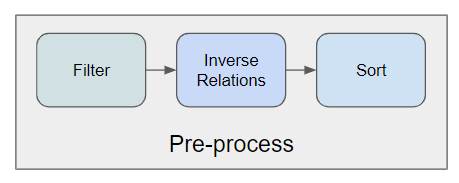
\includegraphics[width=0.5\linewidth]{imagenes/Preprocess.png}
        \caption{Pre-processing workflow}
        \label{fig:preprocess}
\end{figure}

Another important aspect of the system is that it takes compressed files as inputs, and generates compressed output files. 
This is important mainly due to space restrictions. 
The Wikidata dump\footnote{As of February 2020} is $\sim$36GB compressed and $\sim$480GB decompressed.
A pre-processed output file is $\sim$8GB compressed. 

\subsection{Filter}

The first pre-processing task is to filter the input data. 
We will focus on Wikidata labels and descriptions in the English language. 
We will also remove triples with datatype values or external IDs.
While this step could be optional depending on the use-case, the RDFExplorer system that we currently support does not consider such values, and filtering them, currently helps to reduce the number of triples that the system will have to index later. 
Multiple filtering criteria are implemented in the system. 
At the current development stage, these criteria are hard-coded, but they could be extended to use regular expressions or other types of filtering rules. We have left this as a point of future work.

We include triples that match the following rules in our data:
\begin{itemize}
    \item Where \textit{subject} starts with \texttt{http://www.wikidata.org/entity/}.
    \item Where \textit{predicate} starts with \texttt{http://www.wikidata.org/prop/direct/} 
            \subsubitem and \textit{object} starts with \texttt{http://www.wikidata.org/entity/}.
        \subitem or \textit{predicate} is \texttt{label}, \texttt{description} or \texttt{alt-label} 
            \subsubitem and \textit{object} is \textit{literal} and ends with \texttt{@en}.
\end{itemize}

\begin{example}
We now present some examples of both filtered and non-filtered triples.
We have used prefixes when required for shortening lines.

Examples of triples that are kept:
\begin{minted}{SPARQL}
#Entity or Property Subject, Label predicate in english:
wd:Q27 rdfs:label "Ireland"@en .
#Entity or Property Subject, Description predicate in english:
wd:Q147 schema:description "young of a cat"@en .
#Entity or Property Subject, Alternative Label predicate in english:
wd:P22 skos:altLabel "dad"@en .
#Entity subject, Property predicate, Entity subject triples:
wd:Q465 wdt:P277 wd:Q251 .
\end{minted}

Examples of triples that are removed:
\begin{minted}{SPARQL}
#Non-english literal objects:
wd:Q27 rdfs:label "Irlanda"@it .
#Non -Label, -Description or -AltLabel predicates:
wd:Q298 skos:prefLabel "Chile"@en .
wd:Q348 <http://www.wikidata.org/prop/direct-normalized/P349> <object> .
#Non-Entities or -Property subjects:
<http://wikiba.se/beta#Dump> <http://schema.org/softwareVersion> "0.1.0" .
<https://www.wikidata.org/wiki/Special:Entity/Q27> rdfs:label "Irland"@en .
#Non-literal or -entity objects:
wd:Q47 wdt:P1082 "1852168"^^<http://www.w3.org/2001/XMLSchema#decimal> .
\end{minted}
\end{example}

\subsection{Inverse relations and sorting}

Following the filtering process, the system adds the inverse relation for triples patterns containing non-literal objects. 
For every \texttt{(subject, predicate, object)} triple with only non-literal \texttt{objects}, the system adds the inverse \texttt{(object, inverse/Predicate, subject)} triple. This will allow us to treat the subject and object positions of triples equally for the purposes of generating suggestions, while requiring minimal additional code in later components.

\begin{example}
For example, the following triples:

\begin{minted}{SPARQL}
<uri:/subjectA> <uri:/type> <uri:/subjectTypeB> .
<uri:/subjectA> <uri:/predicate> <uri:/objectC> .
\end{minted}

Produces a new file with the original triples, plus the new inverse relation triples:

\begin{minted}{SPARQL}
<uri:/subjectA> <uri:/type> <uri:/subjectTypeB> .
<uri:/subjectA> <uri:/predicate> <uri:/objectC> .
[...]
<uri:/subjectTypeB> <uri:/inverse/type> <uri:/subjectA> .
[...]
<uri:/objectC> <uri:/inverse/predicate> <uri:/subjectA> .
\end{minted}

The separation $[...]$ between \textit{subject}, \textit{object} and \textit{subjectType} statements are due to the final pre-processing task: sorting the output dump file. 
This keeps entity related triples grouped together, which in turn makes indexing more efficient.

\end{example}

The second benefit of this approach, is that with this sorting, finding if an \textit{entity} is a \textit{type} is immediate, since it will contain predicates as \textit{/inverse/type} within its triples. 
The pre-processing could exclude this step; nevertheless, adding the inverse triples significantly reduces indexing time, while without it, several iterations through disk access would have been required. 

The final step is to sort the pre-processed file. Sorting is done via merge sort. At the current development stage, the process is called from the command line. It is to be noted that for sorting of the file, $\sim$3$\times$ the size of the input file is required as free disk space. The command used for sorting is as follows: 

\begin{minted}[frame=none]{bash}
    gzip -dc {input} | LANG=C sort                      \
         -S 200M                                        \
         --parallel=4                                   \
         -T tmp/                                        \
         --compress-program=gzip | gzip > {output}
\end{minted}

This command takes an \texttt{\{input\}} compressed file as parameter. It sorts it using the \texttt{tmp/} folder for storing temporary files, where each chunk during the merge-sort process is as large as 200 Mbytes. During the process, it uses 4 threads. Finally the sorted results are compressed to an \texttt{\{output\}} file.

% ##############################################################################################
% ##############################################################################################
% ##############################################################################################

\section{Index}
\label{chap:index}

After a pre-processed dump has been created, the system can start indexing it. 
Indexing occurs in two steps: once for entities and once for properties. In the end, two indexes are created, one for each.

Entity indexing involves the following steps:
\begin{itemize}
    \item Rank entities via PageRank
    \item Index entities
\end{itemize}

Properties indexing has the following steps:
\begin{itemize}
    \item Rank properties by frequency
    \item Build a domain dictionary
    \item Build a range dictionary
    \item Index properties
\end{itemize}

A depiction of both of these processes can be seen in \autoref{fig:indexing}.

\begin{figure}[H]
    \centering
        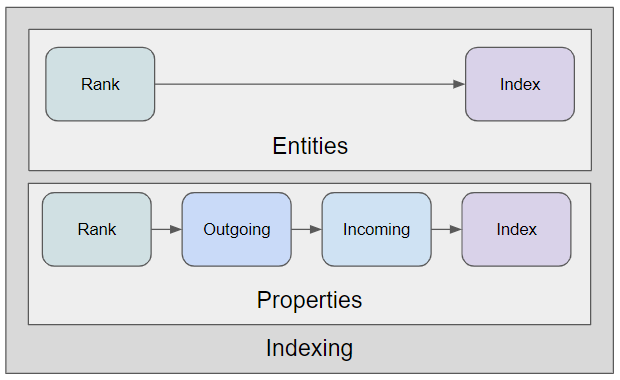
\includegraphics[width=0.7\linewidth]{imagenes/Indexing.png}
        \caption{Indexing workflow}
        \label{fig:indexing}
\end{figure}

\subsection{Entities}

\subsubsection{Inverted Index}

Data relating to entities is indexed using \textit{Lucene}. 
As discussed in \autoref{chap:lucene}, Lucene is a search engine library, mostly suitable for text indexing and searching capabilities. 
This enables out-of-the-box keyword-search for entities and properties.
As mentioned previously, Lucene adds an additional relevance metric based on TF-IDF, which complements the PageRank value that we will calculate later.

The index in Lucene is a document database index. 
Each document of this database has fields. 
In our case, each document corresponds to an \textit{Entity} and each \textit{Entity} has fields such as \textit{Label}, \textit{Description} or a collection of \textit{Properties}. 
We now present each \textit{Field} that every Document in our index has, and the description of those \textit{Fields}.

Each entity-document contains the following fields:
\begin{itemize}
    \item \textbf{Id:} String field. The IRI of the entity. In our case, it is stored without the prefix. For Wikidata, this identifier is a letter \texttt{Q} followed by the identification number.
    \item \textbf{Label:} Text field.  Value that represents a name for the resource (that may be ambiguous).  In the Wikidata dump, the label is the value of the triples with the predicate \url{http://www.w3.org/2000/01/rdf-schema#label}. 
    \item \textbf{AltLabel:} Text field. Other names the resource is known by.  The predicate for these values in the dump is \url{http://www.w3.org/2004/02/skos/core#altLabel}. This field can store multiple values for the same document.
    \item \textbf{Description:} Text field. Small description of the resource, which helps to disambiguate the resource from others with the same or similar labels. Triples with a description have the predicate \url{http://schema.org/description}.
    \item \textbf{InstanceOf:} String field. Indicates if the entity is a type. For example, \textit{Barack Obama (Q76)} is type \textit{Human (Q5)}. \textit{Human} has a \textit{InstanceOf} field with a \textit{"true"} value while \texttt{Barack Obama} has an InstanceOf field with \textit{"false"}.. This is based on having a property \texttt{inverse/instanceOf (P31)} on at least one incoming edge. This is possible due to adding the previously mentioned inverse relation for properties in the pre-processing stage, which when sorted groups both incoming and outgoing edges for a particular entity.
    \item \textbf{Property:} String field. The collection of the outgoing properties that this resource has. This field can store multiple values. All values in this field are stored without their prefix. Property predicates start with  \url{http://www.wikidata.org/prop/direct/}
    \item \textbf{InverseProperty:} String field. Same as the Property field, but for incoming properties. As was mentioned before, these triples were added in the pre-processing step to the dump file.
\end{itemize}

\subsubsection{Ranking}

Lucene offers relevance-based ranking (using a variant of TF-IDF) for searches. But we need importance too: a user might be searching for the term `Obama'. The reader might think about \textit{Barack Obama} as a first suggestion; though \textit{Tom Obama} or \textit{Mount Obama} might have the same relevance in terms of TF-IDF and keywords, one result is much more important than the other and thus we assume it to be of higher prior probability to be relevant to the user.

In order to get the results sorted by both relevance and importance, a ranking value, calculated via PageRank, is added to our index. 
As seen in \autoref{chap:pagerank}, PageRank was originally designed for directed graphs such as websites and their links. 
PageRanks works by iteratively setting relevance values on nodes based on the incoming and outgoing nodes (edges pointing to other nodes). 
In the same way, our PageRank implementation works by iteratively setting the relevance of incoming and outgoing entities through their edges. 

Our implementation of PageRank works in memory, and is not different from other implementations. 
Due to the amount of data, for our implementation we have considered using value types (e.g.: \texttt{int, double, arrays}) instead of more complex reference types (e.g.: \texttt{List, Dictionary, etc.}) in favor of performance. 
Twenty iterations have been considered for this ranking process.

PageRank values are stored in the index as \textit{Lucene's Boost} value. This helps Lucene to sort the results of a query by their importance, as well as relevance. PageRank values are stored in both the \textit{Label} and \textit{AltLabel} fields.

\begin{example}
As an example, a collection of triples from a single entity is presented. Its indexed document and field representation is also presented. We have taken a partial sample of the Universe (Q1) as an example reference.

\begin{minted}{SPARQL}
wd:Q1 schema:description "totality of space [...]"@en .
wd:Q1 rdfs:label "Universe"@en .
wd:Q1 skos:altLabel "Our Universe"@en .
wd:Q1 skos:altLabel "The Cosmos"@en .
wd:Q1 wdt:P31 wd:Q36906466 .
wd:Q1 wdt:P361 wd:Q3327819 .
wd:Q1 wdt:P793 wd:Q323 .
wd:Q1 wdt:P828 wd:Q323 .
wd:Q1 <http://www.wikidata.org/prop/reverse/P1542> wd:Q323 .
\end{minted}

The index document representation for this triples is shown in \autoref{table:triplesToDocument}.

\begin{table}[h!]
\centering
\begin{tabular}{ll}
Field           & Value                    \\ 
\hline
Id              & Q1                       \\
Label           & Universe                 \\
AltLabel        & Our Universe             \\
AltLabel        & The Cosmos               \\
Description     & totality of space [...]  \\
InstanceOf      & Q36906466                \\
Property        & P361                     \\
Property        & P793                     \\
Property        & P828                     \\
InverseProperty & P1542                   
\end{tabular}
\caption{Document and field representation of example triples describing the universe}
\label{table:triplesToDocument}

\end{table}

\end{example}

\subsection{Properties}
The next step in the initialization stage is to create an index for the properties contained in the input dataset.

\subsubsection{Inverted Index}
As  was done with the \textit{Entities Index}, an \textit{index} for the \textit{properties} in the dump is also created. In this case, each document corresponds to a \textit{property} and each \textit{property} has fields such as \textit{label}, \textit{description} or a collection of \textit{domain} and \textit{ranges}. 
We now present each \textit{field} in our index, and the properties of those \textit{fields}.

Each property-document contains the following fields:
\begin{itemize}
    \item \textbf{Id:} String field. The IRI of the property. In our case, it is  stored without the prefix. For Wikidata, this identifier is a letter \texttt{P} followed by the identification number.
    \item \textbf{Label:} Text field.  Value that represents a name for the resource.  For the properties in the dump, the same predicate (\url{http://www.w3.org/2000/01/rdf-schema#label}) is used for labels. 
    \item \textbf{AltLabel:} Text field. Other names the resource is known by. The predicate for these values in the dump is \url{http://www.w3.org/2004/02/skos/core#altLabel}. As in the entities index, this field can store multiple values for the same document. Frequency relevance values are stored here as well. This helps Lucene to sort the results of a query by their relevance.
    \item \textbf{Description:} Text field. Small description of the resource, which helps to disambiguate the resource from others with the same labels. Triples with a description have the predicate \url{http://schema.org/description}.
    \item \textbf{Domain:} String field. The collection of the entity-types with one or more instances that have one or more edges with the given property directed outwards from them. This field can store multiple values. All values in this field are stored without their prefix.
    \item \textbf{Range:} String field. The collection of the entity-types with one or more instances that have one or more edges with the given property directed inwards towards them. This field can store multiple values. All values in this field are stored without their prefix.
\end{itemize}

\subsubsection{Ranking}
For ranking \textit{Properties}, the frequency of appearance is used as our relevance metric. 
We are using frequency since PageRank, which is good for ranking nodes in a directed graph, is not very good for ranking edge labels.
In order to calculate these values, a \textit{Dictionary} is built with the \textit{Key} being the \textit{PropertyId} and the \textit{Value} being the amount of times this property appears in the dataset.

Frequency relevance values are used as \textit{Lucene's Boost}, which are multiplied with the reference scores computed based on TF-IDF. This helps Lucene to sort the results of a query by relevance. The Boost values are added again to both \textit{Label} and \textit{AltLabel} fields.

\subsubsection{Type Domains}

Given a triple pattern statement, \textit{Type Domains} allow the system to provide suggestions in the following two scenarios:
\begin{itemize}
    \item Given a \textit{Property}: the system provides suggestions for the \textit{Subject}.
    \item Given a \textit{Subject}: the system provides suggestions for the \textit{Property}.
\end{itemize}

\textit{Type Domains} work by creating a \textit{Dictionary} with \textit{PropertyId} as \textit{Key} and all the \textit{TypeIds} that each \textit{Property} has as \textit{Domain}.

\begin{example}
Given the following data:
\begin{minted}[frame=none,linenos=false]{SPARQL}
<uri:/BarackObama> <uri:/instanceOf> <uri:/Human> .
<uri:/BarackObama> <uri:/bornIn> <uri:/Honolulu> .
\end{minted}

And given the following triple pattern:
\begin{minted}[frame=none,linenos=false]{SPARQL}
?var1 <uri:/bornIn> ?var2 .
\end{minted}

As suggestions for \texttt{?var1} the system provides instances of \texttt{Human} as suggestions, sorted by relevance. Among the results \texttt{BarackObama} can be found.

This type of query usually times out when run on the remote endpoint (when no or a not low enough \texttt{LIMIT} statement is present) and will not offer ranked options. Our claim is that this feature of our system will provide users with ranked suggestions in a predictable amount of time.
\end{example}

\begin{example}
Given the following data:
\begin{minted}[frame=none,linenos=false]{SPARQL}
<uri:/BarackObama> <uri:/instanceOf> <uri:/Human> .
<uri:/BarackObama> <uri:/bornIn> <uri:/Honolulu> .
\end{minted}

And given the following triple pattern:
\begin{minted}[frame=none,linenos=false]{SPARQL}
<uri:/BarackObama> ?prop1 ?var2 .
\end{minted}

As suggestions for \texttt{?prop1} the system provides properties that direct outwards from instances of \texttt{Human}, sorted by frequency. Among the results \texttt{bornIn} can be found.

It is worth mentioning that for this scenario, the baseline system queries the remote endpoint, which returns the properties only available for \texttt{BarackObama}. In case that this query fails, our system would do as mentioned before and return the approximated results from our local index.
\end{example}

\subsubsection{Type Ranges}

Given a triple pattern statement, type ranges allow our system to provide suggestions in the following two scenarios:
\begin{itemize}
    \item Given a \textit{Property}: the system provides suggestions for the \textit{Object}.
    \item Given an \textit{Object}: the system provides suggestions for the \textit{Property}.
\end{itemize}

\textit{Type Ranges} work in a similar way as \textit{Type Domains}: by creating a \textit{Dictionary} with \textit{PropertyId} as \textit{Key} and all the \textit{TypeIds} that each \textit{Property} has as \textit{Range}.

\begin{example}
Given the following data:
\begin{minted}[frame=none,linenos=false]{SPARQL}
<uri:/BarackObama> <uri:/bornIn> <uri:/Honolulu> .
[...]
<uri:/Honolulu> <uri:/instanceOf> <uri:/City> .
\end{minted}

And given the following triple pattern:
\begin{minted}[frame=none,linenos=false]{SPARQL}
?var1 <uri:/bornIn> ?var2 .
\end{minted}

As suggestions for \texttt{?var2} the system provides instances of \texttt{City} as suggestions, sorted by relevance. Among the results \texttt{Honolulu} can be found.

This type of query times out on a SPARQL endpoint in most cases. As in the \textit{Type Domain} example, we claim that this indexed feature will once again provide users with ranked suggestions in a predictable amount of time.
\end{example}

\begin{example}
Given the following data:
\begin{minted}[frame=none,linenos=false]{SPARQL}
<uri:/BarackObama> <uri:/bornIn> <uri:/Honolulu> .
[...]
<uri:/Honolulu> <uri:/instanceOf> <uri:/City> .
\end{minted}

And given the following triple pattern:
\begin{minted}[frame=none,linenos=false]{SPARQL}
?var1 ?prop1 <uri:/Honolulu> .
\end{minted}

As suggestions for \texttt{?prop1} the system provides properties that point to instances of \texttt{City}, sorted by frequency. Among the results \texttt{bornIn} can be found.

In contrast to what was described for the type domains, our experience has shown that these values are not always returned before a timeout from the remote endpoint since in Wikidata, objects such as cities, countries, types, etc., may have very high in-degree. This feature of our system will provide users ranked suggestions in a predictable amount of time.
\end{example}

\section{Query Parser}
\label{chap:parser}

Once both entities and properties have been indexed, the system can go into online mode. After receiving a user request, the first action of the system is to parse the given request.

We have previously mentioned that the system can work in two ways: keyword search and query term suggestions. Keyword search is quite straightforward: a keyword is given and the inverted index searches and returns the relevant values. These requests go directly to the inverted index, which in turn returns the desired results. No further processing is involved.

Regarding the query term suggestions, there are two possible inputs that the system can take:
\begin{itemize}
    \item \textbf{Query as a graph:} A graph object is passed to our system. This integrates better with graphical user interfaces, such as RDFExplorer.
    \item \textbf{Query as text:} A SPARQL query is passed to our system. This approach is most suitable for text query clients, such as the Wikidata Query Endpoint.
\end{itemize}

For both query term suggestion cases, the goal of the \textit{Query Parser} is to convert the input into a graph data model.

In SPARQL query input scenarios, the input query text is converted using the following triple pattern rules:
\begin{itemize}
    \item Only \texttt{SELECT WHERE} queries are supported in the current version. The system will ignore the \texttt{SELECT} variables (since suggestions can be generated for both projected and unprojected variables when building the query) and take the \texttt{WHERE} statements.
    \item Each triple pattern statement follows a \texttt{Subject Predicate Object} construction.
    \item Each term can be either a constant or a variable.
    \item Each variable will start with the question mark character \texttt{?}. E.g.: \texttt{?var1, ?prop7}
    \item Each constant can be either an IRI in the form of \texttt{<http://iri>} or \texttt{prefix:iri}, when the prefix is given.
\end{itemize}

Given such inputs, parsing an incoming request is straightforward and the queries are converted to the input graph.

% ##############################################################################################
% ##############################################################################################
% ##############################################################################################

\section{Graph Exploration}
\label{chap:graph_exploration}

After a request has been received and the data has been converted into the graph data model, the system explores this graph to check existing relations between nodes and edges. 

The first step of the graph exploration process checks the following:
\begin{itemize}
    \item Which nodes and edges are variables and which are constants.
    \item Which variable nodes have an \texttt{instanceOf} outgoing edge.
\end{itemize}

As a first step, all edges are marked as constant or variable: 
if an edge has a URI as its property, then that edge is considered constant; otherwise it is considered to be variable. 
All nodes are checked in the same manner: if a node has a provided URI, then that node is considered to be a constant, otherwise it is considered to be a variable. 

The next step is to mark the variable nodes as \texttt{Typed}:
If a node is the source of an \texttt{instanceOf} property edge with a target constant, then the node is considered to be \texttt{typed}. To expand on this, let us consider the following statement: \texttt{?var1 instanceOf Human}. As a remark for this case, no other incoming and outgoing edges are available for \texttt{?var1}. We can then consider \texttt{?var1} to have the type \texttt{Human}.

We can summarize this graph exploration with the pseudo-code shown in \autoref{fig:codeExploration}.
\begin{figure}[H]
\begin{minted}[]{csharp}
ExploreGraph (graph) {
  //We will start by the edges:
  foreach (edge in graph.Edges) {
    //If the edge has a given URI, then it is a constant:
    if (edge.Property.IsURI())
      edge.IsConstant = true;
    //If the URI is instanceOf, then we mark it as such:
    if (edge.Property.IsInstanceOfURI())
      edge.IsInstanceOf = true;
  }
  //Then with nodes, same as before:
  foreach (node in graph.Nodes) {
    if (node.IsURI())
      node.IsConstant = true;
    //Now we check the outgoing edges.
    //If any outgoing edges is InstanceOf, then the node is also:
    foreach (outEdge in node.OutgoingEdges)
      if (outEdge.IsInstanceOf && outEdge.TargetNode.IsURI())
        node.IsTyped = true;
  }
}
\end{minted}
\caption{Pseudo-code used to exploring if edges and nodes are constants or instance of a type.}
\label{fig:codeExploration}
\end{figure}

As the last step we check if the input query has enough valid information. We first check if the input is conformed by multiple disconnected sub-graphs. If so, we evaluate each disconnected sub-graph to find if any constants are given in that sub-graph. Consider the following example: 
\begin{minted}[frame=none,linenos=false]{SPARQL}
?v1 ?p1 ?v2 . 
?v2 ?p2 ?p3 .
\end{minted}
In the two statements, only variables and no constants are provided.
Since a plethora of values could be returned for this sub-query, our system avoids this sub-graph and lets the remote SPARQL endpoint decide a selection of values that should be returned in such cases.

The graph exploration allows us to annotate certain nodes and edges, and consider them valid for query execution. To summarize the different exploration scenarios:
\begin{itemize}
    \item Nodes and edges are classified as constants or variables: if a node or edge is a constant, then we do not return any suggestions for it.
    \item Nodes are classified as \texttt{typed}.
    \item Edges are classified as \texttt{instanceOf}.
    \item \texttt{Typed} nodes with no other incoming or outgoing edges are directly queried over our local index.
    \item Sub-graphs with only variables are directly queried over the SPARQL endpoint.
\end{itemize}

Once all nodes and edges have been annotated, our system will proceed to evaluate the graph query and fetch the suggestions. 

% ##############################################################################################
% ##############################################################################################
% ##############################################################################################

\section{Query Execution}
\label{chap:execution}

The goal of our Query Execution module is to get results for our graph's variable nodes and edges, which become suggestions for the user. The results will be retrieved from either the local index or the remote endpoint, but a request will be sent to both, with priority on the remote endpoint. In other words, we will query the remote endpoint for exact results: if it times out, the local approximated results will be returned.

Before diving into the details of how the results are retrieved, we will present an example that covers what we have seen so far and what comes ahead.

\begin{example}

Let us consider the "siblings that have directed a film together" example given in \autoref{fig:siblingsQueryGraph} and the query written for it in \autoref{fig:siblingsSPARQL}.

Building such a query in a Visual Query Builder, such as RDFExplorer; or directly into the Wikidata Query Service, will time out since the graph pattern is quite complex and has many variables that can match millions of nodes in the data. We recall that our goal in such a scenario is to provide users with over-approximated suggestions, so that they can assign values to the variables until the query does not time out and the correct results are provided.

Let us go through how our system will process this query. 
As a first step, our system will explore the graph to retrieve information about it using the algorithm described in \autoref{fig:codeExploration}:
\begin{minted}[frame=none]{text}
n1, n2 are constants (Film, Human);
e1, e2, e3 are constants (instanceOf);
?movie is an instance of type Film;
?human1, ?human2 are instances of type Human;
\end{minted}

Our proposals for the \texttt{?movie}, \texttt{?human1} and \texttt{?human2} variables are currently limited to the information available in our index for instances of those types: instances of Human and Film. As readers might suspect, there are millions of values that these individual variables can take in Wikidata. The suggestions for entities are unlikely to be of relevance because the query is still to broad.

Our system in this case will support users in narrowing the options for the rest of variables: the properties, which in turn support our users in completing the missing information in the graph.

Looking at the graph, we can make the following observations:
\begin{minted}[frame=none]{text}
?director has domain Film and range Human;
?sibling has domain and range Human;
\end{minted}

Our index contains the domain- and range-types for all properties, from here we know: for each type, the incoming and outgoing properties. 
We can use this information at this point to annotate that each variable-property must be both in the incoming-properties for the target-node-type and the outgoing-properties for the source-node-type.

Let us ground this last paragraph with some focus on our given example. Let us focus on \texttt{?director}. The following is noted by our system:

\begin{minted}[frame=none]{text}
?director has source ?movie and target ?human1;
?movie is instance of type Film;
Type Film has a collection of outgoing properties: FilmOutProps;
FilmOutProps could be properties like: director, filmedIn, nominatedFor;

?human1 and ?human2 are instances of type Human;
Type Human has a collection of outgoing properties: HumanOutProps
Type Human has a collection of incoming properties: HumanInProps;
HumanOutProps could be properties like: sibling, bornIn, workLocation;
HumanInProps could be properties like: sibling, namedAfter, director;

?director must be in the intersection of FilmOutProps and HumanInProps;
?sibling must be in the intersection of HumanInProps and HumanOutProps;
\end{minted}

Using the previous process, we can now provide a list of proposals to our users:
\begin{minted}[frame=none]{text}
?director: [producer, director, actor, ...]
?sibling: [motherOf, fatherOf, sonOf, siblingOf, ...]
\end{minted}

At this stage, a user can select their desired property from the suggestions. 
Every time new information is added to the query graph, the query is sent to the remote SPARQL endpoint, in our case Wikidata. 
Since more properties and entities are now assigned and fewer results need to be handled in general, the query will eventually not time out and the exact results will be provided to the user.

\end{example}

It is worth mentioning that, since we do not know if the remote endpoint will time out, both queries are sent in parallel threads. The remote endpoint query is sent right before the graph exploration. 
In our experience while testing our system, we have observed that some user queries can be sent to the remote SPARQL endpoint and the response can come in a fraction of a second, while others can take minutes, or even time out. 
We have run several tests with different values and the response time can vary significantly for the same query at different times. We will explore query times in more detail in section~\autoref{chap:evaluation}.

In this section we will go into more detail about how both queries are built and sent. First, the details of the remote endpoint requests are revised, before discussing the local index.

\subsection{Remote Endpoint Requests}

As was mentioned before, after processing the user query, it is sent to the remote endpoint. Since the focus is on enriching the user experience, in order to send the queries to the remote endpoint, the query is first simplified.

During our tests we have realized that using services such as the \textit{Wikidata Label Service}, or querying for labels, can dramatically increase the query response time and time out for several queries. In order to overcome this and provide the users with useful information about the queried entities, the label and description for all the endpoint results are retrieved from the local index.

Finally, filters and operators that may exist in the query are removed. While we acknowledge that this can have an impact on the intent of the query, we have considered that this could be included in future versions of the system, and it is not included for now.

The following modifications are handled:
\begin{itemize}
    \item A query will be sent for each disconnected sub-graph.
    \item Both labels and descriptions for each element are added from the local index.
    \item Filters and operators are removed from the query.
\end{itemize}

With the previous conditions at hand, the system will send the request to the endpoint and wait for the response.

\subsection{Access to Local Index}

For the local specialized index, additional graph exploration is required. The goal is: if a property is constant, project the property's domain- and range-types onto the adjacent variable-nodes; if the node is constant then project its properties onto incoming- and outgoing-variable-properties; otherwise if the node is typed, project the properties with those node types in their domain and range onto the incoming- and outgoing-variable-properties.

We previously presented the example  "siblings that have directed a film together" (\autoref{fig:siblingsQueryGraph}): we covered the high-level process of how suggestions are made for variables given some constants and \texttt{instanceOf} edges. We explained how by providing suggestions, users could complete their queries with approximate suggestions until the remote endpoint returned exact results before time out. 

In this section, we are going to explain in more detail how we do our final graph exploration and which results we will get from our local index. For this, we will start with a simple graph pattern and later progress to a more complex one.

\begin{example}
Let us consider the graph of \autoref{fig:example_graph1}.

\begin{figure}[H]
    \centering
        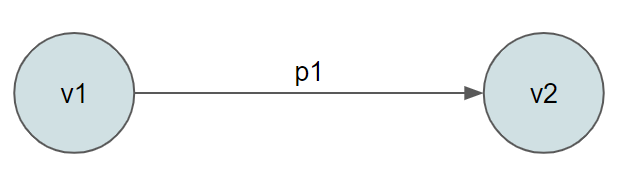
\includegraphics[width=0.5\linewidth]{imagenes/graph1.png}
        \caption{Local index access for a simple graph.}
        \label{fig:example_graph1}
\end{figure}

The graph on \autoref{fig:example_graph1} can be described by the following triple pattern: \texttt{v1 p1 v2}. We consider that each term may be constant or variable. If all of the elements are variables, we would let the remote endpoint handle this case (as was described in \autoref{chap:graph_exploration}). For this reason, we will assume that something in this graph is a constant: \texttt{v1}, \texttt{p1} or \texttt{v2}.

Let us consider that \texttt{p1} and \texttt{v2} are variable, but \texttt{v1} is constant. Moreover, let us consider that \texttt{v1} is known to be an instance of type \texttt{Human}.

Let us also consider that we have the following data in our index:
\begin{minted}{csharp}
human1.Properties = [favoriteFood, gender, ...]
human1.Type = [Human]
[...]
human2.Properties = [studiedAt, bornIn, ...]
human2.Type = [Human]
\end{minted}

From the information above, we also know the following for our type \texttt{Human}:
\begin{minted}{csharp}
Human.OutgoingProperties = [favoriteFood, gender, studiedAt, bornIn, ...]
Human.IncomingProperties = [namedAfter, president, author, ...]
[...]
\end{minted}

Given this information, we could provide our users suggestions for \texttt{p1}. This includes properties such as \texttt{favoriteFood}, \texttt{gender}, \texttt{bornIn}, among others.

\end{example}

The previous case shows how we can provide property suggestions for users with no knowledge about the existing structure of a dataset. We would also like to highlight what we have mentioned before about approximated results: since our index is not storing individual triples, but relationships between types, we could provide suggestions that might not be in the original dataset.

Additional to what we could suggest for \texttt{p1}, and given that we have a collection of possible results for \texttt{p1}, we could also infer certain information about the types for \texttt{v2}: instances of the range types for the previous properties, e.g.: instances \texttt{Food}, \texttt{Gender} or \texttt{City}, sorted by relevance.

While this can be costly, the amount of properties in for a large dataset such as Wikidata is around 1300\footnote{The total number of properties are around 8000, but those going from entity-to-entity are only 1300. Other properties go to strings or other datatypes.}, which limits the possibilities for each domain to a few hundred at most. We have decided to also calculate the possible inferred types for \texttt{v2} in this process, since this allow us to provide users with approximate information while building their queries. 

As a summary, for a \texttt{v1 p1 v2} triple pattern, where \texttt{v1} is constant, the following occurs:
\begin{itemize}
    \item The incoming and outgoing properties of all types are indexed.
    \item \texttt{p1} is an outgoing property of the type of \texttt{v1}.
    \item \texttt{v2} is an instance of the range of one of the possible properties for \texttt{p1}.
\end{itemize}

Readers might notice that the previous reasoning would also apply if only \texttt{v2} is constant: we would be able to get suggestions for both \texttt{p1} and \texttt{v1}.

\begin{example}
In the same graph as before, let us now consider that only \texttt{p1} is constant e.g.: \texttt{bornIn}. From our index, we can retrieve both the domain and range for \texttt{bornIn}. 

Let us consider the following values in our index:
\begin{verbatim}
    bornIn.Domain = [Human, Monster, Star, ...]
    bornIn.Range = [City, Hospital, Dungeon, SolarSystem, ...]
\end{verbatim}

Our system will provide suggestions for \texttt{v1} that are instances of \texttt{Human}, \texttt{Monster} or \texttt{Star}, sorted by relevance. The same will occur for \texttt{v2}: instances of \texttt{City}, \texttt{Hospital} or \texttt{Dungeon} could be proposed.

\end{example}

As a summary, for a \texttt{v1 p1 v2} triple pattern, where \texttt{p1} is constant, the following occurs:
\begin{itemize}
    \item The domain and range of all properties are indexed.
    \item \texttt{v1} is an instance of one of the classes in the domain of \texttt{p1}
    \item \texttt{v2} is an instance of one of the classes in the range of \texttt{p1}
\end{itemize}

In our previous example we covered the simplest of all cases. Now we would like to generalize: any node has multiple incoming and outgoing edges.

\begin{example}

Let us consider the graph of \autoref{fig:example_graph2}. 

\begin{figure}[h]
    \centering
        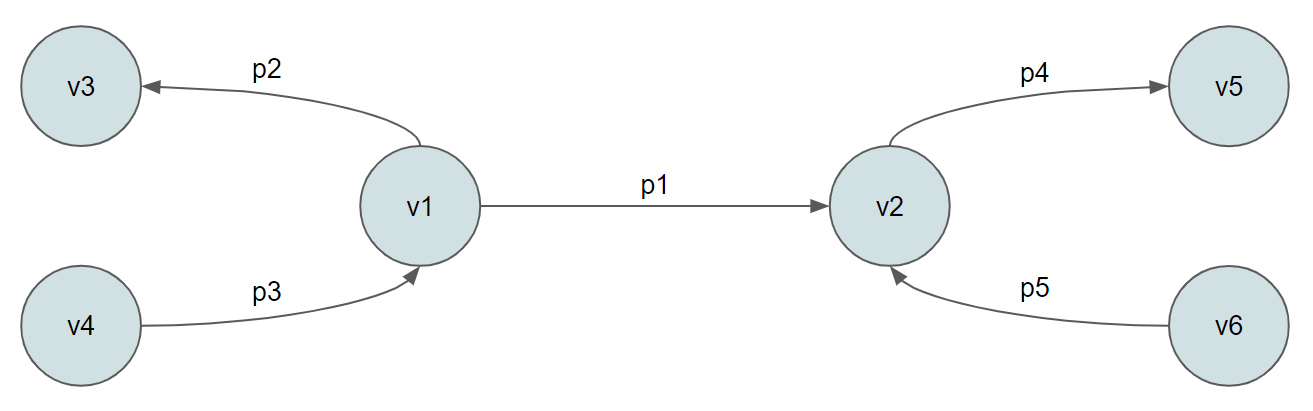
\includegraphics[width=\linewidth]{imagenes/graph2.png}
        \caption{Example graph for expanding domain- and range-types.}
        \label{fig:example_graph2}
\end{figure}

We will consider that any number of elements (nodes or properties) are constant. For each of these constants, we will propagate their types: nodes will contribute with their types to adjacent variable properties; properties will contribute with their domain- and range-types to subject and object variable nodes.

Our first step will be to expand known types among neighbours. The pseudo-code in \autoref{fig:codeExpandNodes} and \autoref{fig:codeExpandEdges} depicts how this task is done for both nodes and properties (i.e., edge labels).

\begin{figure}[h]
\begin{minted}[]{csharp}
// Input:  A query graph with triples as edges;
// Output: The query graph with annotated types for nodes;
//         We will use them to populate our domain and range types (Figure 4.14) 
//         and our edge suggestions (Figure 4.16).
// We refer by DB to our Index database;
ExpandNodes(graph) {
  //We first expand node types:
  foreach(node in graph.Nodes){
    if(node.IsConstant)
      // The DB.GetTypes() method, will query our DB
      // for types (eg.: given Felix, will return Cat)
      node.Types = DB.GetTypes(node);

    //Get types from instanceOf-edges:
    else if(node.IsTyped) 
      // This GetTargetNodeTypes() method will get all types
      // for the instanceOf edges of a node.
      // eg.: given: node - instanceOf - Cow; will return Cow.
      // This applies for multiple instanceOf edges of the node.
      node.Types = graph.GetTargetNodeTypes(node);
  }
}
\end{minted}
\caption{Pseudo-code for expanding node types.}
\label{fig:codeExpandNodes}
\end{figure}

For properties, more logic is required. Checking if the property is constant is not enough, since for example \texttt{bornIn} can have domain \texttt{Human}, \texttt{Cat}, \texttt{Dog}, etc. and range \texttt{City}, \texttt{Hospital}, \texttt{Country}, etc. If in the graph, a specific source type is given, then that type is used instead of the domain, thus further narrowing the available types.

\begin{figure}[h]
\begin{minted}[]{csharp}
// Input:  A query graph with triples as edges;
// Output: The query graph with annotated domain and range types on edges;
//         We will use them to populate our node types (Figure 4.15)
// We refer by DB to our Index database;
ExpandEdges(graph) {
  foreach (edge in graph.Edges) {
    property = edge.Property;
    source = edge.Source;
    target = edge.Target;

    //Source domain types first:
    if(source.IsConstant || source.IsTyped)
      // if the source is given, then the domain are 
      // the types of the source node.
      edge.DomainTypes = source.Types;
    else if(property.IsConstant)
      // Otherwise, get the domains from the DB.
      edge.DomainTypes = DB.GetPropertyDomains(property);

    //Then target range types.
    if(target.IsConstant || target.IsTyped)
      // if the target is given, then the range are 
      // the types of the target node.
      edge.RangeTypes = target.Types;
    else if(property.IsConstant)
      // Otherwise, get the types from the DB.
      edge.RangeTypes = DB.GetPropertyRanges(property);
  }
}
\end{minted}
\caption{Pseudo-code for expanding edge domain- and range-types.}
\label{fig:codeExpandEdges}
\end{figure}

Once we have all known types in place, we can now get values for both nodes and edges. For nodes, we will focus on the outgoing and incoming edges. From these edges, we collect: for the outgoing edges, the domain types (our node must be inside this domain); and for the incoming edges, we collect the range types (our node must also be in this range). In other words, we are going to intersect the outgoing-edges-domain-types and the incoming-edges-range-types. A high-level detail of this process can be appreciated in \autoref{fig:codeResultsNodes}.

\begin{figure}[h]
\begin{minted}[]{csharp}
// Input:  A query graph with triples as edges;
// Output: The query graph with annotated results for suggestions of instances on nodes;
// We refer by DB to our Index database;
GetNodesResults(graph){
  foreach (node in graph.Nodes){
    // We already know what it is, we do not propose suggestions
    if(node.IsConstant) continue;
        
    if(!node.IsTyped) {
      // In practice we initialise types with the types from one of the edges.
      // We present it this way for simplicity.
      node.Types = DB.GetAllTypes();
      
      foreach (outEdge in node.outEdges) {
        if(outEdge.DomainTypes.IsNotEmpty())
            node.Types = Intersect(node.Types, outEdge.DomainTypes);
      }
      foreach (inEdge in node.inEdges) {
        if(inEdge.RangeTypes.IsNotEmpty())
            node.Types = Intersect(node.Types, inEdge.RangeTypes);
      }
    }
    // Finally we get instances for our types.
    // If our node is of a given type, we get instance values:
    // node.IsType = Cat --> node.Results = Simon, Felix, Grumpy, etc.
    // Results will be sorted by relevance and importance.
    node.Results = DB.GetInstancesOf(node.Types);
  }
}
\end{minted}
\caption{Pseudo-code for expanding edge domain- and range-types.}
\label{fig:codeResultsNodes}
\end{figure}

For edges (\autoref{fig:codeResultsEdges}), we will focus on both the source- and target-node of our edges. We first do some checks on if these nodes are constants or instances of another type. If either our source or target nodes are constant, then we have certainty of the possible values that our edge can have (we recall that we have added these values directly into our DB).

If the source or target node is an instance of another type (thus a variable), then we query the outgoing or incoming properties for that type: while indexing, we have collected these properties for all instances of that type. But in this case, we also explore other possible relations existing in our graph.

Focusing on each node, we will check all outgoing edges with constant properties. Being constant, the properties on these edges can provide information about the values for their domains, and with these, the type of our node. We intersect the domains for all such properties. We will do the same for the incoming edges with constant properties of our source node. If there are such incoming edges, then our node type must be in the range of each of those properties, and thus we again intersect the ranges. Finally, after getting approximate results for both our nodes and edges, a list of entities and properties are now available. 

\begin{figure}[h]
\begin{minted}[]{csharp}
// Input:  A query graph with triples as edges;
// Output: The query graph with annotated results for suggestions of properties on edges;
// We refer by DB to our Index database;
GetEdgesResults(graph){
  foreach(edge in graph.Edges){
    property = edge.Property;
    // We already know what it is, we do not propose suggestions.
    if(property.IsConstant) continue;
    
    source = edge.SourceNode;
    target = edge.TargetNode;

    suggestions = new Set();
    // Properties of the instance (Like outgoing properties for Barack Obama);
    sourceProps = DB.GetOutgoingProperties(source);
    targetProps = DB.GetIncomingProperties(target);
    // Properties of the Type (like outgoing properties of Type Human);
    domainProps = DB.GetPropertiesWithDomainIn(source.Types);
    rangeProps = DB.GetPropertiesWithRangeIn(target.Types);
    if (source.IsConstant && target.IsConstant) {
      suggestions = Intersect(sourceProps, targetProps);
    } else if (source.IsConstant) {
      suggestions = sourceProps;
    } else if (target.IsConstant) {
      suggestions = targetProps;
    } else {
      // In Figure 4.15 we added all types for nodes that had no constants or types.
      suggestions = Intersect(domainProps, rangeProps);
    }
    edge.Results = suggestions;
  }
}
\end{minted}
\caption{Pseudo-code for expanding edge domain- and range-types.}
\label{fig:codeResultsEdges}
\end{figure}

\end{example}

Something else that must be mentioned is that for remote queries: both the label and the description are retrieved from the local index and the results are returned to the user. 

% ##############################################################################################
% ##############################################################################################
% ##############################################################################################

\subsection{Approximations}

We have discussed how our system provides suggestions to our users, but we would like to cover the scenario where our system will provide over-approximated results.

\begin{example}
Let us consider the following data:

\begin{minted}[frame=none,linenos=false]{SPARQL}
<uri:/SeattleSlew> <uri:/instanceOf> <uri:/Horse> .
<uri:/SeattleSlew> <uri:/winner> <uri:/KentuckyDerby> .
# [...]
<uri:/Seabiscuit> <uri:/instanceOf> <uri:/Horse> .
<uri:/Seabiscuit> <uri:/sibling> <uri:/Lottery> .
# [...]
\end{minted}

And given the following triple pattern:
\begin{minted}[frame=none,linenos=false]{SPARQL}
?horse <uri:/instanceOf> <uri:/Horse> .
?horse <uri:/winner> ?race .
?horse ?prop ?object .
\end{minted}


In our sample data, only \texttt{Seattle Slew} has the \texttt{winner} property (and no \texttt{sibling} property), but since our data is indexed based on our domain- and range-types, for \texttt{?prop}, we will also get \texttt{sibling} as a suggestion property, although our data has no triples with both properties there.

\end{example}

% ##############################################################################################
% ##############################################################################################
% ##############################################################################################

\section{Application Interface}
\label{chap:api}

The last module of our system is the application interface. It will allow our system to take requests from front-end clients and use our backend.

As was mentioned before, our system supports several types of requests:
\begin{itemize}
    \item Keyword search for entities.
    \item Keyword search for properties.
    \item Keyword search for types.
    \item Get information about a Q-code entity: label, description, etc.
    \item Get information about a P-code property: label, description, etc.
    \item Query term with a SPARQL query text.
    \item Query term with a graphical representation of a SPARQL query.
\end{itemize}

The keyword search directly reverts to the specialized index. The query term works as was previously described in this chapter.

With all of these components in place, our backend can accept and respond to requests from a frontend client. In the following chapter we will describe how to integrate our system with RDFExplorer as the client in order to apply our approach for a concrete use-case.


\chapter{Use case}
\label{chap:Frontend}

As a proof of concept, we have integrated our backend with a user interface. 
Originally we planned to build one from scratch, but while doing our research on the state of the art, we stumbled upon several existing alternatives. 
A very interesting one is RDFExplorer, developed by Vargas et al.~\cite{Vargas2019}. 
In their design, Vargas et al. propose a language and a visual interface that allow users to build and execute graph-based queries in an intuitive way. 
Their claim is that their work allows non-expert users to express graph-pattern queries better than existing interfaces with similar expressiveness. 

In this chapter we will focus on the proof of concept of our design: 
providing users query-term suggestions while they are building SPARQL queries. 
That said, while we are using RDFExplorer as our user interface, any user interface that would provide users suggestions for their SPARQL query building process would be a valid candidate.

We will start by describing the RDFExplorer system and some issues it exhibits while providing suggestions, mainly because of the way it gets suggestions directly from the Wikidata endpoint results. 
We will then proceed to describe an integration with our backend API to get better response times while parallelizing access to both our local specialized index and the remote endpoint.

\section{RDFExplorer}

RDFExplorer is a query building interface that allows users to visually create queries by adding entities and properties as they would add nodes and edges in a graph. The following is an example of a query built via RDFExplorer. In it, \texttt{?var1} refers to instances of \texttt{human} with \texttt{place of birth} in \texttt{Honolulu}.

\begin{figure}[h]
    \centering
        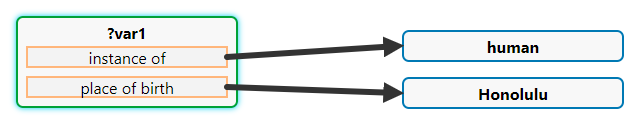
\includegraphics[width=.8\linewidth]{imagenes/rdfExplorer1.png}
        \caption{Building a query with RDFExplorer.}
        \label{fig:rdfExplorer1}
\end{figure}

In the process of building the graph of \Cref{fig:rdfExplorer1}, users can go through the state of \Cref{fig:rdfExplorer_nearTimeout}. 
In this intermediate state neither \textit{place of birth} nor \texttt{Honolulu} are yet given. 
In fact, this might be a very common state in the initial queries built by users, where they construct the graph structure of the query and then look to replace variables with specific constants. 

\begin{figure}[h]
    \centering
        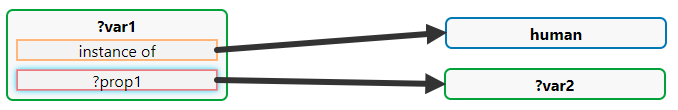
\includegraphics[width=0.8\linewidth]{imagenes/near timeout query.png}
        \caption{Getting suggestions for \texttt{?prop1} takes around 45 seconds on direct queries to the Wikidata Endpoint.}
        \label{fig:rdfExplorer_nearTimeout}
\end{figure}

In order to get results, RDFExplorer will construct a query based on the graph that the user is visually building, send a request to the remote endpoint and await for results: in our case, the Wikidata SPARQL endpoint. 
It is to be noted that this is not the query that is shown in the user interface, but the one that is sent to the endpoint\footnote{As appears in the browser's developer tools}. 
For our example, the graph in \Cref{fig:rdfExplorer_nearTimeout} is represented by the following SPARQL query:

\begin{minted}{SPARQL}
PREFIX wdt: <http://www.wikidata.org/prop/direct/>
PREFIX wd: <http://www.wikidata.org/entity/>
PREFIX wikibase: <http://wikiba.se/ontology#>
PREFIX rdfs: <http://www.w3.org/2000/01/rdf-schema#>
SELECT DISTINCT ?prop1 ?prop1Label WHERE {
  ?var1 ?prop1 ?var2 .
  FILTER isIRI(?var2)
  ?var1 wdt:P31 wd:Q5 .
  ?prop1tmp wikibase:directClaim ?prop1 .
  OPTIONAL {
    ?prop1tmp rdfs:label ?prop1Label .
    FILTER (lang(?prop1Label) = "en")
  }
} LIMIT 10
\end{minted}

One of the issues that users of the current version of RDFExplorer face, is that suggestions directly from the Wikidata remote endpoint can take a long time, or even time out. For example, the suggestions for \textit{?prop1} in \Cref{fig:rdfExplorer_nearTimeout} take around 45 seconds to return, which is not the best user experience while building queries. It is also important to consider that the user might change, add or remove any of the edges and nodes during that time, with which the query will change and be re-sent to the endpoint, resulting in users having no suggestions that allow them to properly explore a dataset. 

In other cases such as in \Cref{fig:rdfExplorer_timeout}, the results will never return if the user asks for suggestions for \texttt{?prop4}, as the underlying query will require a join that generates a very large number of intermediate results. Such queries can be encountered frequently as users will commonly create various nodes to represent the initial structure of their query and then begin to replace variables with the terms they require. 

\begin{figure}[h]
    \centering
        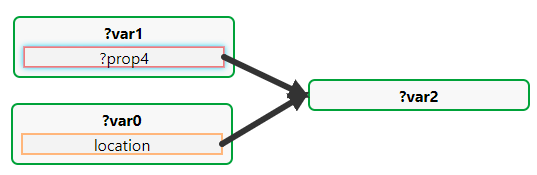
\includegraphics[width=0.7\linewidth]{imagenes/timeout query.png}
        \caption{A timeout query on RDFExplorer.}
        \label{fig:rdfExplorer_timeout}
\end{figure}

One of the issues that our research is trying to solve, in the context of user interfaces such as RDFExplorer, is to enable users to navigate through RDF datasets in almost real-time\footnote{Less than 3 seconds}, while also not limiting the results to 10, but to 100 for backend queries. We do this by approximating results as was seen in \Cref{chap:Backend}.

Our focus during this integration is to compare how different endpoints affect response times. It is not in our focus to make changes to the RDFExplorer interface.

% ##############################################################################################
% ##############################################################################################
% ##############################################################################################

\section{Integration as proof of concept}

In this section we present our backend integration to the RDFExplorer frontend client. The RDFExplorer original source code is currently hosted on github: \url{https://github.com/hvarg/RDFExplorer}. The source code is written in \textit{JavaScript}. We forked this repository\footnote{Forked to \url{https://github.com/gabrieldelaparra/RDFExplorer}} and did our integration in this branch. 

Some code changes were required for our integration: 
\begin{itemize}
    \item Replace the Wikidata endpoint with our local backend.
    \item Replace the request: instead of a SPARQL query, send the graph JSON object.
    \item Convert the response from our backend to the RDFExplorer expected response format.
\end{itemize} 

To get into the details of our integration, we will start by showing the existing architecture of RDFExplorer in \Cref{fig:uiBeforeRequests}. In it, we can see how the system is originally directing its request directly to the Wikidata Endpoint. 

\begin{figure}[h]
    \centering
        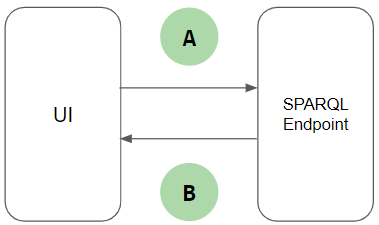
\includegraphics[width=0.4\linewidth]{imagenes/uiBeforeRequest.png}
        \caption{Requests before integration}
        \label{fig:uiBeforeRequests}
\end{figure}

The requests and responses were originally sent as SPARQL queries and the Wikidata API was in charge of returning results as a JSON data object. Both the requests and responses depicted by \texttt{A} and \texttt{B} in \Cref{fig:uiBeforeRequests} are detailed in \Cref{table:uiBeforeRequest}.

\begin{table}[h]
\centering
\begin{tabular}{ll}
Action & Data \\ 
\hline
A              
& \begin{minipage}[t]{0.85\linewidth}
\begin{minted}{SPARQL}
PREFIX ...
SELECT ... 
WHERE {
  ?s ?p ?o .
  FILTER isIRI(?o)
  ?p_tmp wikibase:directClaim ?p .
  OPTIONAL {
    ?p_tmp rdfs:label ?label .
    FILTER (lang(?label) = "en")
  } 
} 
LIMIT 10
\end{minted}
\end{minipage}
\\ \\ \\
B             
& \begin{minipage}[t]{0.85\linewidth}
\begin{minted}{json}
{"head" : 
  { "vars" : 
    [ "prop1", "prop1Label" ] 
  },
"results" : {
  "bindings" : [ {
    "prop1" : {
      "type" : "uri",
      "value" : "http://www.wikidata.org/prop/direct/P611"
    }, 
    // other bindings/variables
  }  ]  }}
\end{minted}
\end{minipage}
\\
\end{tabular}
\caption{UI and Endpoint interactions before our integration.}
\label{table:uiBeforeRequest}
\end{table}

After our integration, the system architecture is as seen in \Cref{fig:uiAfterArchitecture}. It can now be seen that the system directs its requests to our backend, where the requests are parallelized to both our local specialized index and to the remote Wikidata endpoint.

\begin{figure}[h]
    \centering
        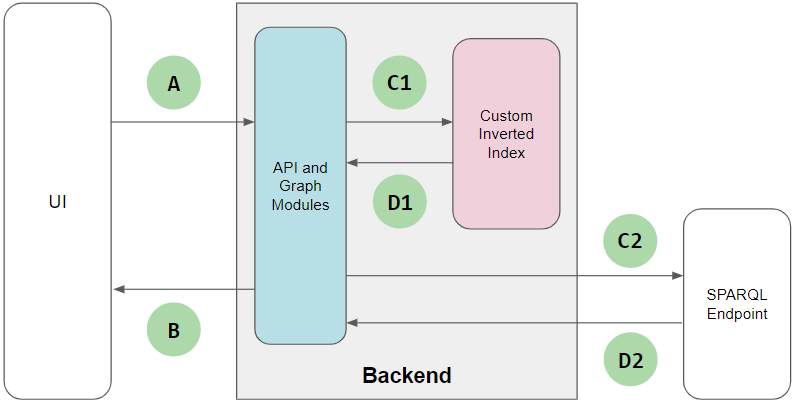
\includegraphics[width=\linewidth]{imagenes/uiAfterRequest.png}
        \caption{Architecture and requests after integration}
        \label{fig:uiAfterArchitecture}
\end{figure}

As can be seen in \Cref{table:uiAfterRequest1} and \Cref{table:uiAfterRequest2}, the requests and responses in this integration have changed. The most important changes are as follows:
\begin{itemize}
    \item \texttt{A:} The UI now sends a JSON object of the query graph.
    \item \texttt{B:} Our response has changed from the original Wikidata response. We now send a different JSON Object.
    \item \texttt{C1} and \texttt{D1} are internal, so no requests and responses are sent; nevertheless, they are shown in the schema for reference.
    \item \texttt{C2:} Is a SPARQL basic graph pattern.
    \item \texttt{D2:} Is the same Wikidata response. The results from either D1 or D2 will be parsed by our system and converted to \texttt{B} depending on the timeouts set and the response times encountered.
\end{itemize}
 
\begin{table}[h]
\centering
\begin{tabular}{ll}
Action & Data \\ 
\hline
A              
& \begin{minipage}[t]{0.85\linewidth}
\begin{minted}{json}
{"nodes": [ {
  "id": 0, "name": "var0",
  "uris": [ ]
  },
  // other nodes
],
"edges": [ {
  "id": 0, "name": "prop0",
  "uris": [],
  "sourceId": 0, "targetId": 1
  },
  // other edges
]}
\end{minted}
\end{minipage}
\\ \\ \\
B             
& \begin{minipage}[t]{0.85\linewidth}
\begin{minted}{json}
{"nodes": [ {
  "id": 0, 
  "suggestions": {
   "Q2": {
     "label": "Earth",
     "uri": "http://www.wikidata.org/entity/Q2"
    }, 
    // other suggestions
    } 
  },
  // other nodes
  ], 
"edges": [ 
  // edges with suggestions
  ]}
\end{minted}
\end{minipage}
\\
\end{tabular}
\caption{UI and Backend interactions after our integration.}
\label{table:uiAfterRequest1}
\end{table}


\begin{table}[h]
\centering
\begin{tabular}{ll}
Action & Data \\ 
\hline
C2             
& \begin{minipage}[t]{0.85\linewidth}
\begin{minted}{SPARQL}
PREFIX ...
SELECT ... 
WHERE {
  ?s ?p ?o .
  FILTER(STRSTARTS(STR(?s), "wd:") .
  FILTER(STRSTARTS(STR(?p), "wdt:") .
  FILTER(STRSTARTS(STR(?o), "wd:") .
} 
LIMIT 100
\end{minted}
\end{minipage}
\\ \\ \\
D2             
& \begin{minipage}[t]{0.85\linewidth}
\begin{minted}{json}
{"head" : 
  { "vars" : 
    [ "prop1", "prop1Label" ] 
  },
  "results" : {
    "bindings" : [ {
      "prop1" : {
        "type" : "uri",
        "value" : "http://www.wikidata.org/prop/direct/P611"
      }, 
    // other bindings/variables
    }  ]  }}
\end{minted}
\end{minipage}
\\
\end{tabular}
\caption{Backend and Endpoint interactions after our integration.}
\label{table:uiAfterRequest2}
\end{table}

Without going into the code nuances for our integration, we rather provide some high-level details on the changes required for our integration. 

Regarding \texttt{A}, originally RDFExplorer sent a SPARQL request to the Wikidata Endpoint, but internally handled a graph object. We considered that using the graph model, which is one step above before the graph-to-SPARQL conversion, could be more flexible for future integrations, so we started our integration there.

The RDFExplorer graph model is a common graph implementation, and also very similar to the one that we are using. In fact, the RDFExplorer implementation has more data values for nodes and edges, which we do not require and thus trimmed for the request. The graph model using for the requests is based on the following structure:
\begin{minted}{json}
{"nodes" : { "id", "uris"[ ], "name" },
 "edges" : { "id", "uris"[ ], "name", "sourceId", "targetId" }}
\end{minted}

Some additional changes, while not required, are that we now check whether the graph  changes during the query construction. Originally, the RDFExplorer UI will send a new request for any changes in the node/edge coordinates or selection. While this is not required, it improves the overall performance since changes to the nodes positions do not trigger a new request now. 

The response that we return in \texttt{B} has also changed. Initially RDFExplorer is waiting for a JSON response from Wikidata. Our integration response will include all the data required by the UI, but with some changes in the structure. 

The response from our system is as follows:
\begin{minted}{json}
{"nodes": { "id", "values": [ { "uri", "label" }, ... ], ... },
 "edges": { "id", "values": [ { "uri", "label" }, ... ], ... }}
\end{minted}

With these changes in place, our RDFExplorer client can now query to our local endpoint and give users suggestions while building SPARQL queries in the graph-based user interface.

The remaining \texttt{C2} and \texttt{D2} work just as they had previously worked from Wikidata to the UI, but this time, the requests and responses are handled by our backend and converted from and to the previously mentioned data structures.

As was mentioned in \Cref{chap:execution}, we will send two queries to both indexes: via \texttt{C1} to our local index and via \texttt{C2} to the remote endpoint. If we receive a response from the remote endpoint (\texttt{D2}) within a configurable timeout threshold, we return these remote endpoint exact results, otherwise if the remote endpoint times out, we return our local approximated results (\texttt{D1}).

\chapter{Evaluation}
\label{chap:evaluation}

In this research we have built a specialized inverted index to support users during dataset exploration and SPARQL query building tasks on large-scale RDF datasets. In this chapter we present an evaluation of both the indexing and querying processes described in this work. We will start by posing some questions that our evaluation will address:

\begin{itemize}
    \item How long does the indexing process take?
    \item How much space does indexing require?
    \item How are our times compared against SPARQL endpoint query times?
    \item How do our approximation suggestions compare to precise results?
\end{itemize}

In order to answer these questions, we will first present the experimental settings used for this research.

\section{Experimental setup}

For this work, we have used a personal computer with an i7-4600M CPU @ 2.9 GHz and 16 GB of RAM, running on Windows 10.

We based our development on the Wikidata dump of March 4\textsuperscript{th} 2018 (20,821,216,963 bytes); and our evaluation of the system with the dump of May 23\textsuperscript{rd} 2020 (41,285,029,233 bytes). We had originally developed results from our first Wikidata dump, but we found out that the information in our dataset was outdated, and as a consequence, that results against the Wikidata query service were too different to compare.

Regarding the source code, it was written in C\# and tested with \textit{xUnit} with 217 tests and 89\% code coverage. As external packages we have used the following:
\begin{itemize}
    \item For logging, we use \textit{NLog} (v.4.5.10)
    \item \textit{dotnetRDF} (v.2.2.0) is used for RDF handling
    \item For Zip file handling we are using \textit{SharpZipLib} (v.1.0.0)
    \item File types (zip or plain text NTriples) are detected using \textit{Mime} (v.3.0.2)
    \item JSON objects are handled via \textit{Newtonsoft.Json} (v.12.0.2)
    \item Sorting of filtered and inverse triples files is done using \textit{gzip} (v.1.9)
\end{itemize}

% ##############################################################################################
% ##############################################################################################
% ##############################################################################################

\section{Index}

In this section we present metrics for both preprocessing and indexing.

The preprocessing phase gave us the following results:

\begin{table}[h!]
\centering
\begin{tabular}{lrl}
Task                                    & Value  &                    \\
\hline
Size of input file                      & 41,285,029 & KBytes       \\
Number of input triples (lines)         & 5,126,548,635  &            \\
Size of output file                     & 9,184,248 & KBytes        \\
Number of output triples                & 1,098,606,588 &             \\
Runtime duration                        & 34:59:22  & hh:mm:ss        \\
\end{tabular}
\caption{Overview of preprocessing in terms of space and time}
\label{table:preprocessingMetrics}
\end{table}

The indexing process has the following metrics:

\begin{table}[h!]
\centering
\begin{tabular}{lrl}
Task                                    & Value  &                    \\
\hline
Number of input triples                 & 1,098,606,588 &             \\
PageRank runtime duration               & 11:16:25 & hh:mm:ss        \\
Entity index runtime duration           & 58:10:11 & hh:mm:ss       \\
Number of entities                      & 84,623,017 &                \\
Size of entity index                    & 9,721,912 & KBytes         \\
Property index runtime duration         & 5:07:50 & hh:mm:ss       \\
Number of properties                    & 7,559 &                     \\
Size of properties index                & 9,992 & KBytes             \\
Total index size                        & 9,731,904 & KBytes         \\
\end{tabular}
\caption{Overview of indexing in terms of space and time}
\label{table:indexMetrics}
\end{table}

% ##############################################################################################
% ##############################################################################################
% ##############################################################################################

\section{Queries}

We have mentioned before that our system will provide over-approximated suggestions. Readers might wonder how can we measure this? In this section, we would like to show how approximated our results are compared to the exact ones provided from the Wikidata SPARQL endpoint. We will use precision and recall to measure how similar our approximated results are to the exact Wikidata results.

For this, we are going to create a list of sample properties and run queries using these. We expect to get an over-approximation of our suggested values, while not leaving any values outside. In other words, we are expecting that we return all true positives while also having a considerable amount of false positives and low-to-zero false negatives: we expect our over-approximation model to have 100\% recall, with any drop in recall being due to changes in the data between our indexing process, and running the queries on the live SPARQL endpoint.

\subsection{Sample queries}
For our queries, we have created a list of sample properties. Selecting a sample set of properties can be a daunting task: what makes a property a good candidate for testing? A straightforward approach would be to randomly sample properties with equal probability, but most properties in Wikidata have very few triples, while those few properties with more triples are more likely to appear in user queries. Hence, the straightforward sampling approach does not seem appropriate. We would rather prefer to have an evaluation set that includes properties with differing numbers of triples (frequency), domain classes and range classes.

We thus decided to create a sample set based on two approaches: random and cherry-picking. Since picking properties randomly could return some not-so-interesting properties (low frequency, domain or range), we followed the following approach: First we sorted the properties randomly; we calculated the total sum of the value (e.g.: Sum of all frequencies) that we were looking for and calculated the cumulative contribution to the total. From that total, we took 10 random values between 0-1: this way, we compute a weighted sample where properties are sampled with a probability proportional to their value. This gives us 30 properties: 10 for frequency, domain and range.

For the cherry-picking approach, we took an additional 37 properties that had a mix of frequency/domain/range values. We manually selected some properties that had values in between the spectrum of values and added them to the previous list, e.g.: We picked P21 (sex or gender) that has a high frequency, a high domain and a low range. Furthermore, P301 (category's main topic) was also picked, which has a high frequency, a low domain and a high range.

We took 67 sample properties in total for our tests. In \Cref{table:sampleProperties1} and \Cref{table:sampleProperties2} we present these. In this table we can observe that there is a mix of high and low values for frequency, domain and range.

\begin{table}[]
\resizebox{\textwidth}{!}{%
\centering
\begin{tabular}{llrrr}
\hline
\multicolumn{1}{l}{\textbf{Prop}} & \multicolumn{1}{l}{\textbf{Label}}  & \multicolumn{1}{l}{\textbf{Freq}} & \multicolumn{1}{l}{\textbf{Domain}} & \multicolumn{1}{l}{\textbf{Range}} \\ 
\hline
P17    & country   & 12418513   & 37642   & 664 \\
P19    & place of birth   & 2460395   & 938   & 3344 \\
P21    & sex or gender   & 6053686   & 2341   & 13 \\
P31    & instance of   & 82929158   & 70082   & 5470 \\
P50    & author   & 8812954   & 2357   & 1019 \\
P102   & member of political party   & 380027   & 116   & 245 \\
P106   & occupation   & 4426526   & 1684   & 1366 \\
P112   & founded by   & 44475   & 3766   & 1378 \\
P127   & owned by   & 386560   & 5262   & 2821 \\
P131   & located in the administrative territorial entity   & 9077756   & 20858   & 3482 \\
P135   & movement   & 49381   & 1358   & 365 \\
P138   & named after   & 252683   & 10147   & 7129 \\
P150   & contains administrative territorial entity   & 76236   & 1155   & 1875 \\
P155   & follows   & 962127   & 8064   & 7955 \\
P156   & followed by   & 955311   & 7837   & 8146 \\
P159   & headquarters location   & 309781   & 5825   & 2390 \\
P180   & depicts   & 151551   & 2134   & 4989 \\
P184   & doctoral advisor   & 24767   & 10   & 16 \\
P276   & location   & 1701029   & 14419   & 4892 \\
P279   & subclass of   & 2427200   & 9631   & 4915 \\
P287   & designed by   & 9745   & 1292   & 242 \\
P301   & category's main topic   & 624932   & 68   & 16273 \\
P361   & part of   & 2137841   & 20309   & 12870 \\
P364   & original language of film or TV show   & 291691   & 552   & 101 \\
P413   & position played on team / speciality   & 337554   & 39   & 62 \\
P421   & located in time zone   & 1491148   & 3004   & 92 \\
P511   & honorific prefix   & 47040   & 61   & 58 \\
P527   & has part   & 551031   & 11313   & 17077 \\
P531   & diplomatic mission sent   & 303   & 4   & 44 \\
P611   & religious order   & 26152   & 319   & 92 \\
P641   & sport   & 1539461   & 7673   & 185 \\
P682   & biological process   & 370975   & 46   & 22 \\
P710   & participant   & 67173   & 1601   & 1639 \\
P793   & significant event   & 107608   & 4342   & 1528 \\
P805   & statement is subject of   & 353   & 201   & 155 \\
P807   & separated from   & 878   & 157   & 171 \\
P873   & phase point   & 23   & 19   & 0 \\
P910   & topic's main category   & 624952   & 16489   & 262 \\
P915   & filming location   & 18844   & 175   & 1334 \\
P921   & main subject   & 7551197   & 3374   & 11388 \\
P971   & category combines topics   & 790631   & 75   & 5702
\end{tabular}}
\caption{Sample properties, part 1}
\label{table:sampleProperties1}
\end{table}

\begin{table}[]
\resizebox{.9\textwidth}{!}{%
\centering
\begin{tabular}{llrrr}
\hline
\multicolumn{1}{l}{\textbf{Prop}} & \multicolumn{1}{l}{\textbf{Label}}  & \multicolumn{1}{l}{\textbf{Freq}} & \multicolumn{1}{l}{\textbf{Domain}} & \multicolumn{1}{l}{\textbf{Range}} \\ 
\hline
P1204   & Wikimedia portal's main topic   & 1654   & 4   & 726 \\
P1344   & participant of   & 240027   & 966   & 1771 \\
P1423   & template's main topic   & 14554   & 21   & 2041 \\
P1424   & topic's main template   & 14095   & 2048   & 46 \\
P1433   & published in   & 35181414   & 1118   & 1008 \\
P1435   & heritage designation   & 1766767   & 7444   & 59 \\
P1445   & fictional universe described in   & 318   & 25   & 197 \\
P1464   & category for people born here   & 34767   & 1295   & 4 \\
P1478   & has immediate cause   & 343   & 156   & 155 \\
P1889   & different from   & 399217   & 10053   & 10019 \\
P2156   & pseudo crystal habit   & 30   & 1   & 0 \\
P2239   & first aid measures   & 698   & 6   & 18 \\
P2522   & victory   & 5644   & 110   & 977 \\
P2614   & World Heritage criteria   & 2717   & 691   & 2 \\
P2860   & cites work   & 7358255   & 937   & 559 \\
P2894   & day of week   & 189572   & 1341   & 12 \\
P3092   & film crew member   & 683   & 21   & 11 \\
P3096   & KML file   & 11125   & 221   & 1 \\
P3259   & intangible cultural heritage status   & 539   & 135   & 8 \\
P3919   & contributed to creative work   & 2451   & 26   & 165 \\
P3985   & supports programming language   & 34   & 21   & 49 \\
P4000   & has fruit type   & 2992   & 22   & 2 \\
P4224   & category contains   & 688147   & 41   & 420 \\
P4599   & monomer of   & 36   & 35   & 6 \\
P4809   & sets environment variable   & 2   & 6   & 1 \\
P4878   & symbolizes   & 17   & 17   & 26
\end{tabular}}
\caption{Sample properties, part 2}
\label{table:sampleProperties2}
\end{table}

With these properties, we will build four types of queries. For each of our properties, we will consider an incoming or outgoing edge from our source or target nodes. We will represent each one of these queries by \texttt{A}, \texttt{B}, \texttt{C} and \texttt{D}, as per the following queries: 

\begin{verbatim}
A: ?v1  p1 ?v2 .    B: ?v1  p1 ?v2 .   C: ?v1  p1 ?v2 .   D: ?v1  p1 ?v2 .
   ?v1 ?p2 ?v3 .       ?v2 ?p2 ?v3 .      ?v3 ?p2 ?v1 .      ?v3 ?p2 ?v2 .
\end{verbatim}

These queries would commonly be encountered as intermediary graphs in query builder interfaces. In each of these four cases, we are going to replace \texttt{p1} with our sample property and query for the values of \texttt{?p2}. This will give us a total of 268 test queries. We will run these queries on both our local index and the remote endpoint without an internal timeout (but still observing the external timeout of 50 seconds from the Wikidata API). We will record both the query execution time on both indexes and the results returned for them both. In the next section we will go into the details of the query execution times and proceed with a comparison of the results from both indexes.

\subsection{Query runtime}

In the previous section we described how we created a collection of 268 sample tests: 4 query types for 67 properties. In this section we compare the query runtime for both our local index and the remote endpoint.

In \Cref{fig:runtimeCompare} a comparison is depicted between our local and remote endpoint query times. In this figure we order the queries by runtime individually for local and remote execution. From these 268 queries, 190 queries, around 70\% of the total, will time out at 50 seconds: the Wikidata Remote Endpoint API timeout; and just 78 queries will return results before the timeout. The local index times cannot be visibly identified, so we have also introduced \Cref{fig:runtimeLocal}.

\begin{figure}[H]
    \centering
        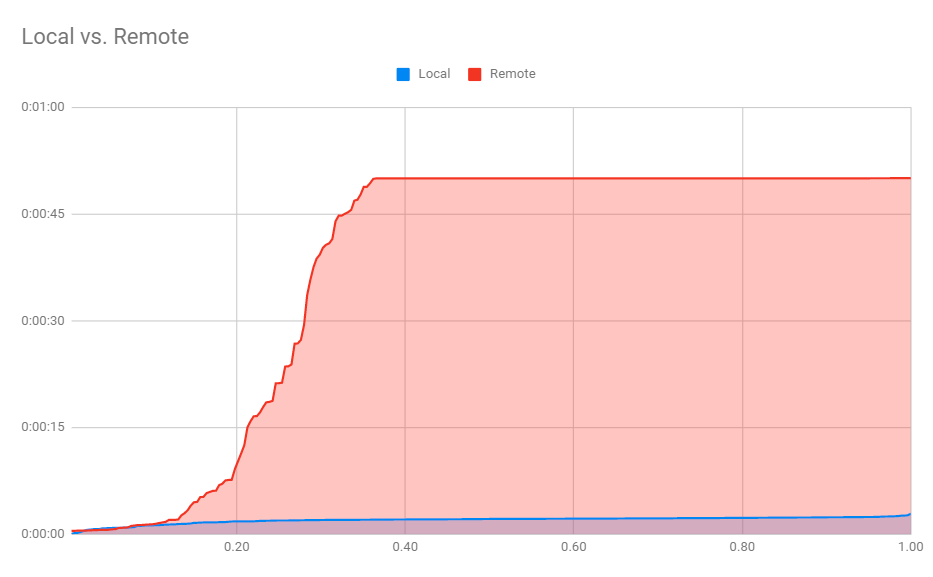
\includegraphics[width=\linewidth]{imagenes/queryRuntimeCompared.png}
        \caption{Comparison of local and remote query times}
        \label{fig:runtimeCompare}
\end{figure}

In our local query times, all queries run in under 3 seconds, with around 8\% running in under 1 second, and 25\% running in under 2 seconds.

\begin{figure}[h]
    \centering
        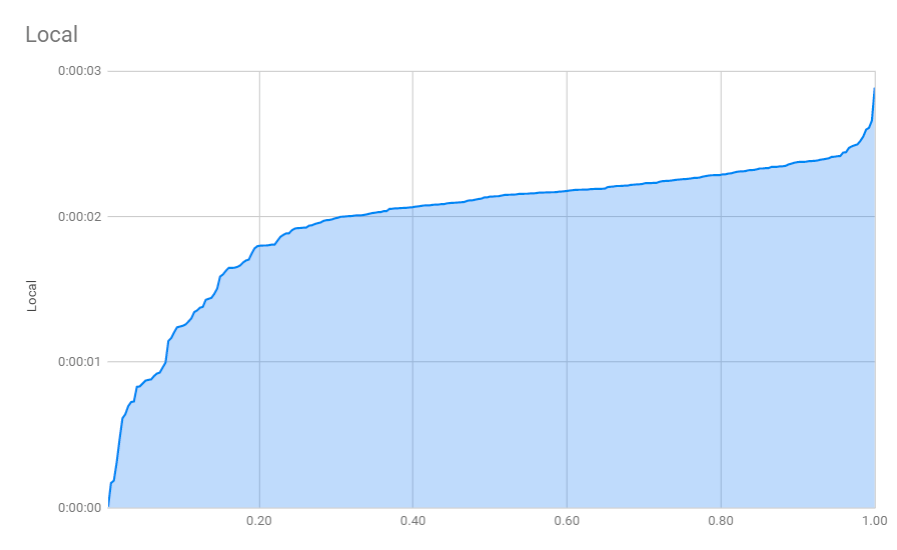
\includegraphics[width=\linewidth]{imagenes/localQueryRuntime.png}
        \caption{Local query times}
        \label{fig:runtimeLocal}
\end{figure}

\subsection{Results approximations}

In our previous section we presented the query runtimes for our 268 queries. In this section we present the results of those queries: How similar are the values that our system suggests compared against the exact values from the remote endpoint? It is worth mentioning that we can only compare  results for the 78 queries that did return values from the remote endpoint. 

For this, we expect to get an over-approximation of our suggested values, meaning that we return all the exact values and some incorrect values as well. 

\begin{figure}[ht]
    \centering
        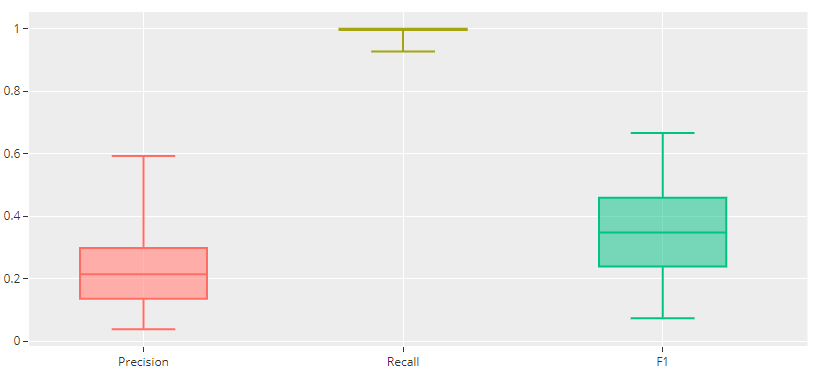
\includegraphics[width=\linewidth]{imagenes/resultsCandleStick.png}
        \caption{Precision, Recall, F1}
        \label{fig:resultsCandles}
\end{figure}

In \Cref{fig:resultsCandles} we present the minimum and maximum results for precision, recall and F1. At the start of this chapter we mentioned that we expected a high value of recall, given that we should suggest all true-positives and that we should not have false-negatives inside our suggestions. The results in this sense are very similar to what we expected: Our results have an average of 99.40\% of recall, where the slight drop in recall is due to changes in the data between our indexing process and querying the live endpoint. Regarding precision: since we are providing over-approximated suggestions, our precision is expected to be low. As an average, we have 22\% precision and 35\% F1.

It is important to note that the results that we can provide are based on the dataset dump, where any changes on the remote endpoint database will not be reflected in our local index. This implies that for any changes in the remote database, our measures will deteriorate in time against the live ones.

% ##############################################################################################
% ##############################################################################################
% ##############################################################################################

\section{Discussion}

We started this chapter by raising some questions about our system performance. Regarding the required time for indexing the Wikidata dump, from our results we can see that indexing is a time-consuming process that can take up to 109 hours to run. Considering that a new dump is generated every week or every two weeks, our system could be scheduled to run after one of the dump generation tasks.

We also considered the space requirements involved for our backend. The system requirements regarding disk space allow our system to keep a version running; sorting our index files requires a peak physical disk space of 300 GB, which is not too demanding for modern hardware.

Comparing our result times and correctness against SPARQL, our system can deliver results within 3 seconds with 25\% precision on average versus exact results. While interactive user suggestions usually can be expected within the milliseconds range, we consider that our 3-second suggestions are acceptable while using the system, especially if compared against the timeouts that most of the tested queries encounter when computed on the remote SPARQL endpoint.

Related to correctness, since our specialized index is built from a dump, which is generated every week, the correctness of the suggestions will gradually reduce: some triples which establish  domain and range relations might be removed or new ones might be added in the online dataset, which in turn generates a difference between our results and the SPARQL endpoint results. This might be avoided by periodically generating a new specialized index, or implementing a delta mechanism to keep the system up to date. This however is out of our current scope.

\chapter{Conclusion}
\label{chap:Conclusion}

This research intends to support users in finding data from the web. More specifically, we intend to help users to explore, navigate and build queries within the Semantic Web context. During the research and development of this project, while learning about the theory and the technology behind, we have collected some observations that we would like to discuss.

Graph databases and especially RDF databases require users to start thinking in terms of graphs or triple patterns. While some may argue that we unconsciously do this all the time, our current data modelling approach is far from naturally expressing ideas and questions in subject-predicate-object triple patterns or other graph data structures.

While this user-to-graph gap is continuously being approached by researchers with works such as: translations between natural language and RDF, ontology mappings, user interfaces or others; there is still a gap between how users think and model relationships within the data and how it is actually stored in RDF datasets.

As an example of this, let us present a simple use case example of how this kind of technology could be used for: It would be interesting to query for songs from a composer that wrote the music for a movie, and search for other albums/songs that were written by the composer. A direct approach to this would be to search (e.g.: Google) for information about the songs, search for the movie, composer and search his works. While this is what most users would probably do, the information about each of these steps can be in different sources: songs could be in Spotify, movies in IMDB, composer in Wikipedia. It is also possible that all the data is already in RDF datasets.

Going for an RDF approach, the first step would be to express the query in s-p-o triple patterns; but there is a second and more important requirement: users need some knowledge about how the data is stored: are songs writtenBy composer or is the composer authorOf a song? Going a bit further, what if the data is structured in a way that the album was writtenBy and the songs are partOf the album? In this case, an additional triple pattern statement is required to properly formulate the query. Situations like these are not naturally understood by users and require some extra work for proper technology adoption.

This work is set in the context where users already understand that they need to express their thoughts in s-p-o triple patterns and that they might need to explore the data in order to understand the existing relationships in the dataset, while possibly needing to invert relations or make assumptions about the data in order to get some answers.

In this existing context, translating user queries into answers (based on RDF data stores), is accessed through SPARQL queries and endpoints. While there are some interesting alternatives to the SPARQL query syntax that could aid users to intuitively build queries, these still rely on SPARQL endpoints, which have some time out issues for retrieving results.

Given this scenario, our goal is to help users navigate through existing large-scale RDF datasets: "which properties exist between different types of entities" or "how are entities linked through properties" are some questions that we would like users to be able to answer while exploring RDF triplestores. In the same context, we would like to provide users with or without any SPARQL syntax knowledge and with little knowledge about the RDF dataset structure to be able to answer these questions.

From our tests and results, we can conclude that our system works according to our expectations: for user-specified graph patterns that would usually timeout in SPARQL endpoints, our system can provide suggestions for both nodes and edges (entities and properties) that can help users complete their queries and get exact results in reasonable time.

In this chapter we are going to cover the main results of our work: 
we will discuss some methods used for our implementation and summarize the main results for both runtimes and correctness. 
We will finish the chapter with certain known limitations and some proposals for future work: 
like in every research work, there are several open questions and paths for improvement. 
While usage and adoption could help identify more use-cases and optimizations, 
we will discuss those points that we currently consider the most relevant.

% ##############################################################################################
% ##############################################################################################
% ##############################################################################################

\section{Main Results}

Our claim is that our system can provide users over-approximated suggestions with full recall in a fraction of the time required to
generate exact results using the remote endpoint. We also expect our system to provide reasonable precision, although some incorrect suggestions will be returned (by which we mean suggestions that, if chosen, will lead to a query generating empty results).

To achieve this we first pre-process and index a large-scale RDF dataset dump, which takes about 109 hours for the 41 GB Wikidata compressed dump with 5,130 million of triples (around 75 seconds for a million triples). The final index output is less than a quarter of the size of the original compressed input: around 9 GB. 

For our indexing engine, we have used Lucene for storage along with PageRank and TF-IDF for sorting our data. This approach allows for out-of-the-box text-based lookups with relevance and importance ordering, while taking advantage of the existing data relationships to prioritize results. For accessing our service, our system is built as a backend that sits between the client's user interface and a remote SPARQL endpoint. Several types of requests can be done: term lookup, query for entity/property Id, input a SPARQL query or input a graph query.

For our tests we have integrated our system with the RDFExplorer visual query builder interface and, as mentioned before, we have indexed the Wikidata dataset dump. To get an understanding of our performance, we have selected 67 properties and generated four types of queries with each, providing 268 test cases. For each test, we run queries in parallel on both the local specialized index and the remote SPARQL endpoint. From the 268 test cases we are only comparing the results for 78 tests: most tests time out on the remote endpoint (50 seconds) and provide no results to compare with. 

The results of these 78 tests show, as we had expected, that our system returns over-approximated results: we achieve a high recall (99.4\% $\sim$ 100\%) and a low precision (0.38\% $\sim$ 59.27\%). Since our methods for indexing avoid the individual triple relations between subject-predicate-object, all local results will be calculated using the types of the entities and this expands the results to all possible triples in the involved types. This explains both the low precision and the high recall. The non-100\% recall is explained due to changes in the Wikidata content after building our local index. We have examined triples from previous dumps and several changes are made to the data: properties are replaced, predicates are modified, added, removed and new relations are constructed. Based on this, it is expected to get a performance degradation as the time passes and the data changes.

Regarding runtime comparisons, we have identified that certain queries, especially those with incoming edges are harder for the remote Wikidata SPARQL endpoint to resolve and usually turn into timeout. This timeout can be handled by setting a limit in user queries, but since our intent was to compare the whole set of results, we left this limit out of the queries. Another point to mention is the response times of our work: while we consider that the results make the user interface usable during query building, 2--3 seconds is quite high for current day standards of millisecond response times and some improvement could be achieved there.

% ##############################################################################################
% ##############################################################################################
% ##############################################################################################

\section{Generalizing this work}
\label{chap:extendingRDF}

While our project has been built using the Wikidata dataset, the proposed techniques can be extended to other RDF datasets. The code has been designed with this in mind and relies on class interfaces for filtering and indexing. These interfaces require implementing the logic to match the URIs and fields of a new RDF dataset.

As an example, we present the code that is used for indexing a label field in Wikidata. Extending this to other datasets should be straightforward: in \Cref{fig:extendingIndex}, line 8 should be replaced with the URI for the label property of the new RDF dataset.

\begin{figure}[H]
\begin{minted}[]{csharp}
public class LabelIndexer : FieldIndexer<TextField> {

  // Here we specify what the label in our index will be.
  public override string FieldName = "Label";

  // With this method, we filter the triples that match our criteria.
  public override bool FilterValidTriples(Triple triple) {
    return triple.Predicate.Uri == "http://www.w3.org/2000/01/rdf-schema#label";
  }

  // With this method, we return the field.
  public override TextField GetField(IEnumerable<Triple> triples) {
    var value = GetFieldValue(triples.Find(FilterValidTriples));
    return new TextField(FieldName, value, Field.Store.YES);
  }

  // With this method, get get the value that we want from the triple.
  public override string GetFieldValue(Triple triple) {
    return triple.Object.LiteralValue;
  }
}
\end{minted}
\caption{For our Wikidata index, we specify our matching criteria. In this case, the predicate for a label field should match the \url{http://www.w3.org/2000/01/rdf-schema\#label} URI. In reality, all strings are constants in a single file to centralize these values.}
\label{fig:extendingIndex}
\end{figure}

We highlight that our techniques are general and do no rely on any specific aspects or optimizations on Wikidata. We think that the results should generalize to other RDF datasets, though further experiments would need to be conducted to confirm this.

Regarding generalizing this project to other user interfaces, the most straightforward way to do this would be to use our server API to request suggestions.
Our API can take a SPARQL query and compute the suggestions for all the variables in the query. The API will return a JSON object with all the queried variables, their labels and URIs.

\section{Limitations and future work}
\label{chap:futureWork}

In this section we present some of our known limitations and some points that we think are open for future work.

The first constraint of our system is that our system currently supports English-only labels and descriptions. While this limitation is easy to overcome, it implies that our pre-processing and indexing process will take longer and in the end, become larger in size. 

Also related to the input triples, we have excluded all triples with datatypes objects (as in subject-predicate-object). We foresee that this could be integrated in our system by adding several additional parent types: \texttt{string}, \texttt{integer}, \texttt{datetime} and so on. In our study of the Wikidata triplestore, we found out that of the 7,559 properties available in Wikidata, only 1,282 or 17\% are used in our system. This has major implications: indexing as was mentioned before (times and size), but also in the query execution times. Having 589\% more properties would definitively impact not only the system performance, but also the queries that involve \texttt{string} types would probably take longer.

Another limitation of our system has to do with complex queries. Currently, our system only takes \texttt{SELECT/WHERE} queries (i.e., basic graph patterns) without nested queries nor filters or optionals, etc. While such features broaden the types of queries that can be expressed in SPARQL, it is not in the scope of our project to process these type of queries, but rather to support users with no SPARQL knowledge in using core features. It is worth noting however that the RDFExplorer interface provides access to the SPARQL query being built, which can be extended manually by the user in order to add such features.

Something that we would like to address in the future is to keep our system up-to-date with the endpoint data. There are several ways that this can be approached: taking diffs from the remote endpoint and updating the data would be an interesting option to consider, since this task could be run on a periodical basis with low runtimes. 

In \Cref{chap:Backend} we discussed how \texttt{?movie ?director ?human} could often be queried by users in the inverted relation form, which generates no results: \texttt{?human ?directed ?movie}. We believe that since our system already contains domain and range types, and calculates suggestions for the correct relation direction, our system could also be used to propose inverse relations that might help users in choosing the right property in certain scenarios.

Another option would be to improve the performance of our code: while several changes could be done to optimize our code to run with the Wikidata triples, we tried not to implement hard-coded rules only valid for that specific dataset, but to make it easy to change the dataset and allow future users to implement their own filtering rules. We also agree that the presented runtimes could be improved with code changes and this would also be one of the future changes that our work could implement.

% \input{glosario.tex} % opcional

\bibliographystyle{plain}
\bibliography{bibliografia}

% \input{anexo_apendices.tex} % opcionales

\end{document}
